% ------------------------------------------------------------------------------
% Mathematics Project Report Template
% by Jon Shiach 2019
% Manchester Metropolitan University
% ------------------------------------------------------------------------------
\documentclass[11pt]{report} 

\usepackage{projectreport}
\usepackage{array} % ragged-right p{} columns in the comparison tables (Chapters 2 and 5)
% Layout aids: let long URLs in the bibliography break anywhere, and give paragraphs a
% little extra stretch so that inline citations do not overflow the text block.
\usepackage{xurl}
\setlength{\emergencystretch}{2em}

% ------------------------------------------------------------------------------
% Enter your details here
% ------------------------------------------------------------------------------
\newcommand{\name}{Hanson Sun}
\newcommand{\course}{BSc. (Hons) Computer Science}
\newcommand{\projecttitle}{Depth-Inference Capable and Robust PhysTwin}
\newcommand{\submissiondate}{May 2026}


% ------------------------------------------------------------------------------
% Document
% ------------------------------------------------------------------------------
\begin{document}

\maketitle

% ------------------------------------------------------------------------------
% Top matter
% ------------------------------------------------------------------------------
\chapter*{Abstract}
PhysTwin is a recent real-to-simulation (real2sim) pipeline that converts RGBD video into a
spring--mass parameterised \emph{warp} digital twin, but it assumes that depth and camera
calibration are already available.

This project presents DIPhysTwin (Depth-Inference PhysTwin), which builds an interactive digital
twin from multi-view RGB video alone. Camera poses and metric scale are recovered with DUSt3R, and
dense depth is inferred with Depth Anything 3 (DA3), which predicts spatially consistent geometry
from arbitrary image sets. In our fixed-camera videos, however, its depth varies between frames.
The available streaming adaptation processes overlapping chunks, but its Umeyama alignment breaks
down on larger chunks; duplicating static views helps only over short windows. The central
contribution of this work is a lightweight temporal depth smoother that learns a residual
correction on top of the DA3 prediction. It needs no ground-truth depth: temporal behaviour is
supervised by a video depth model, while fidelity and edge terms preserve the geometry and
boundaries of the baseline.

DIPhysTwin is evaluated on PhysTwin's released data and on approximately 30 self-recorded
multi-view sessions spanning cloth, mats, bottles, mugs and stuffed animals. It produces working
warp models with pose, depth and ground alignment all inferred rather than measured, and the
quality of the result depends far more on capture conditions than on any single stage: large,
slow-moving objects with little controller occlusion reconstruct well, whereas small, fast-moving
objects lose 3D consistency. The remaining limitations, including the absence of true multi-view
streaming inference, imperfect capture and calibration, and the lack of a robust 3D point tracker,
are analysed and used to outline future work.


\tableofcontents
% \listoffigures
% \listoftables
% \lstlistoflistings		% comment out if not needed

% ------------------------------------------------------------------------------
% Main matter
% Chapters are added to the document using the \include{chapterx} command
% ------------------------------------------------------------------------------
\newpage
\setcounter{page}{0}
\pagenumbering{arabic}
\chapter{Introduction}
\label{cha:introduction}

\section{Motivation and Problem statement}
\label{sec:intro-problem}

Policies for deformable manipulation are learned from recordings of real interactions, and
digitising those recordings by hand takes 3D modelling, material parameters and manual matching. The goal is to automate that process, converting multiple RGB video recordings of the same interaction into a single \emph{digital twin} of the manipulated object.

\textcite{phystwin} proposed PhysTwin, a real2sim pipeline that takes RGBD video from several
cameras, segments the object, tracks the object and the controller, and fits a spring--mass
\emph{warp} model for interaction in NVIDIA Warp \parencite{warp}. This work improves the robustness of PhysTwin by (1) removing the depth sensor, (2) removing camera calibration and (3) tolerating imperfect segmentation and tracking; the resulting pipeline is called DIPhysTwin. It should allow PhysTwin to be used in more flexible capture conditions, with varying degrees of camera setup and less human intervention.

\section{Contributions}
\label{sec:intro-contributions}

The main contributions of this work are:

\begin{enumerate}
	\item \textbf{A depth-inference-first pipeline.} Poses and metric scale come from a dedicated
	stage rather than the depth model, and depth is estimated per view.
	\item \textbf{A ground-truth-free temporal depth smoother.} A small network learns a
	\emph{residual correction} to one depth model's maps, smoothing temporal flicker in depth videos while preserving spatial consistency.
	\item \textbf{Robustness engineering.} The pipeline handles resolutions independently, runs
	idempotently, aligns the scene to the ground with RANSAC and propagates that transform to poses,
	tracks and meshes, with fallbacks when shape prior fitting or dense tracking fails.
\end{enumerate}


 
\chapter{Background and Related Work}
\label{cha:background}

This chapter reviews the core components referenced in the report and identifies the gaps this project addresses.

\section{PhysTwin and Real2Sim Digital Twins}
\label{sec:bg-phystwin}

PhysTwin \parencite{phystwin} takes synchronised multi-view RGBD video of a controller
interacting with an object, segments the object, and tracks dense motion on both the object and
the controller. It lifts those tracks into 3D with depth and trains a spring--mass \emph{warp}
model in NVIDIA Warp \parencite{warp}. The trained model responds to a controller point in the
simulator and reproduces soft-body behaviour.

The PhysTwin pipeline assumes cameras fixed in space while the object and controller(s) move. This assumption complicates multi-view depth reconstruction.

\section{Monocular and Video Depth Estimation}
\label{sec:bg-depth}

VDA \parencite{vda} is a monocular depth model that produces temporally consistent maps for a
single view. Depth Anything 3 (DA3) \parencite{da3} predicts spatially consistent geometry from an
arbitrary number of images, with or without known camera poses. Multi-view input does not by itself ensure
temporal consistency for a moving scene recorded by stationary cameras. In the configuration tested
here, depth varies between frames. The streaming adaptation processes overlapping chunks, but its
Umeyama alignment becomes singular for larger chunks; duplicating the static views as a dynamic
sequence helps only over a limited window (Chapter~\ref{cha:system-design}).

DUSt3R and MASt3R \parencite{dust3r,mast3r} use pairwise 3D correspondences to recover poses.
Their estimates also vary over time in the tested sequences.

As of the current state of research, no model is both spatially and temporally correct. Models that reason over one frame or several
views flicker between frames, while video-consistency models are smooth but geometrically weaker
and monocular (Chapter~\ref{cha:smoother}).

\section{Camera Pose Estimation}
\label{sec:bg-pose}

Intrinsics and extrinsics serve two purposes here: aligning depth maps with the RGB frames used
for segmentation, and triangulating tracked 2D points into 3D tracks. They are not always
measured during capture.

Pose from the depth model was poor in both respects, misaligning 3D projections and degrading
optimisation and training. Empirically, pairwise correspondences from DUSt3R with a heuristic scale aligned
much better (Chapter~\ref{cha:system-design}).

\section{Temporal Depth Stabilisation}
\label{sec:bg-temporal}

VDA \parencite{vda} adds temporal attention at several decoder scales and introduces a temporal
gradient matching (TGM) loss. That loss supervises frame-to-frame \emph{change} in depth rather
than absolute depth, and inference runs over a segment-wise sliding window.

StableDPT \parencite{stabledpt} attends spatially within each frame in the encoder and
temporally across frames in the decoder. It also adopts the TGM loss.

NVDS and NVDS+ \parencite{nvds,nvdsp} stabilise depth after the fact, using sliding-window
cross-attention together with an optical flow model, but they require metric depth.

\begin{table}[H]
	\caption{Comparison of prior temporal depth stabilisation methods}
	\label{tab:bg-temporal}
	\begin{center}
		\begin{tabular}{@{}>{\raggedright\arraybackslash}p{2.2cm}
		                  >{\raggedright\arraybackslash}p{4.6cm}
		                  >{\raggedright\arraybackslash}p{2.4cm}
		                  >{\raggedright\arraybackslash}p{2.2cm}
		                  >{\raggedright\arraybackslash}p{2.4cm}@{}}
			\toprule
			Method & Temporal mechanism & Supervision & Ground-truth depth & Multi-camera input \\
			\midrule
			VDA & temporal attention at multiple decoder scales,
			                      segment-wise sliding window & TGM loss & yes (lidar) & no (monocular video) \\
			StableDPT & spatial attention per frame, temporal
			                      attention across frames in decoder & TGM loss & yes (lidar) & no (monocular video) \\
			NVDS / NVDS+ & post-hoc stabiliser, sliding-window
			                      cross-attention + optical flow & temporal loss via flow
			                      model & yes (sensor ground truth) & no (monocular video) \\
			Li et al. (2023) & not stated & not stated & not stated & not verified \\
			\bottomrule
		\end{tabular}
	\end{center}
\end{table}


All four methods need ground-truth or metric depth, and all four are monocular: each takes a single
video stream and none accepts synchronised views from several cameras. This project
instead needs a smoother for several synchronised views from an uncalibrated capture, trained
\emph{without ground-truth depth} by treating a video depth model (VDA) as a motion oracle.

\section{Dense Tracking and 3D Reconstruction}
\label{sec:bg-tracking}

CoTracker \parencite{cotracker} tracks points jointly rather than independently, which makes it
more stable than pairwise optical flow. It is the tracker the base pipeline uses, and since it
works in 2D, its tracks are lifted into 3D with the estimated depth. Tracking accuracy is
therefore bounded by depth accuracy.

MVTracker \parencite{mvtracker} tracks across several views, SpatialTrackerV2
\parencite{spatrackerv2} tracks in 3D. On the captures used here, the multi-view tracker performed worse than CoTracker and
the 3D tracker produced visible artefacts (Chapter~\ref{cha:evaluation}).

\label{sec:bg-reconstruction}

SAM and its successors \parencite{sam,sam3,groundedsam} produce promptable, open-vocabulary
masks, and their quality depends strongly on how the object is described. Trellis
\parencite{trellis} was evaluated as a source of mesh and shape priors, while appearance is
reconstructed with Gaussian splatting \parencite{gaussiansplatting}.

\section{Summary of the Gap}
\label{sec:bg-gap}

Each area above is well developed on its own, but few models combine the three properties needed here. No widely used
model is spatially consistent, temporally smooth and multi-camera capable at once. Existing
stabilisers need ground-truth depth and are monocular, and most multi-camera reconstruction
assumes a stationary scene with a moving camera, whereas this project observes a moving object
from static cameras.

DIPhysTwin addresses the gap in two ways. The first is a ground-truth-free smoother that
learns a residual correction to flickering depth, with a video model serving only as a motion
oracle (Chapter~\ref{cha:smoother}). The second is a set of robustness measures that let the
pipeline tolerate imperfect input (Chapter~\ref{cha:system-design}).

\chapter{System Design}
\label{cha:system-design}

\section{Pipeline Overview}
\label{sec:design-overview}

DIPhysTwin modifies the data-processing and generation stages of PhysTwin; warp training is unchanged. The new and modified stages are:

\begin{enumerate}
	\item \textbf{DUSt3R pose estimation with heuristic scaling} (new). Camera intrinsics, extrinsics
	      and a metric scale for the scene are recovered here.
	\item \textbf{DA3 depth inference} (new). Dense depth is estimated for every frame of every view
	      with \textcite{da3}.
	\item \textbf{Temporal depth smoothing} (new). A small network learns a residual correction to the
	      DA3 depth maps, which reduces temporal flicker while preserving spatial consistency.
	\item \textbf{Data processing} (modified PhysTwin). Depth maps, masks and images are combined
	      into the per-frame structure the pipeline expects.
	\item \textbf{Extrinsics alignment} (new). The scene is rotated until the ground plane is flat,
	      with everything above it.
\end{enumerate}


\begin{figure}[H]
    \begin{center}
        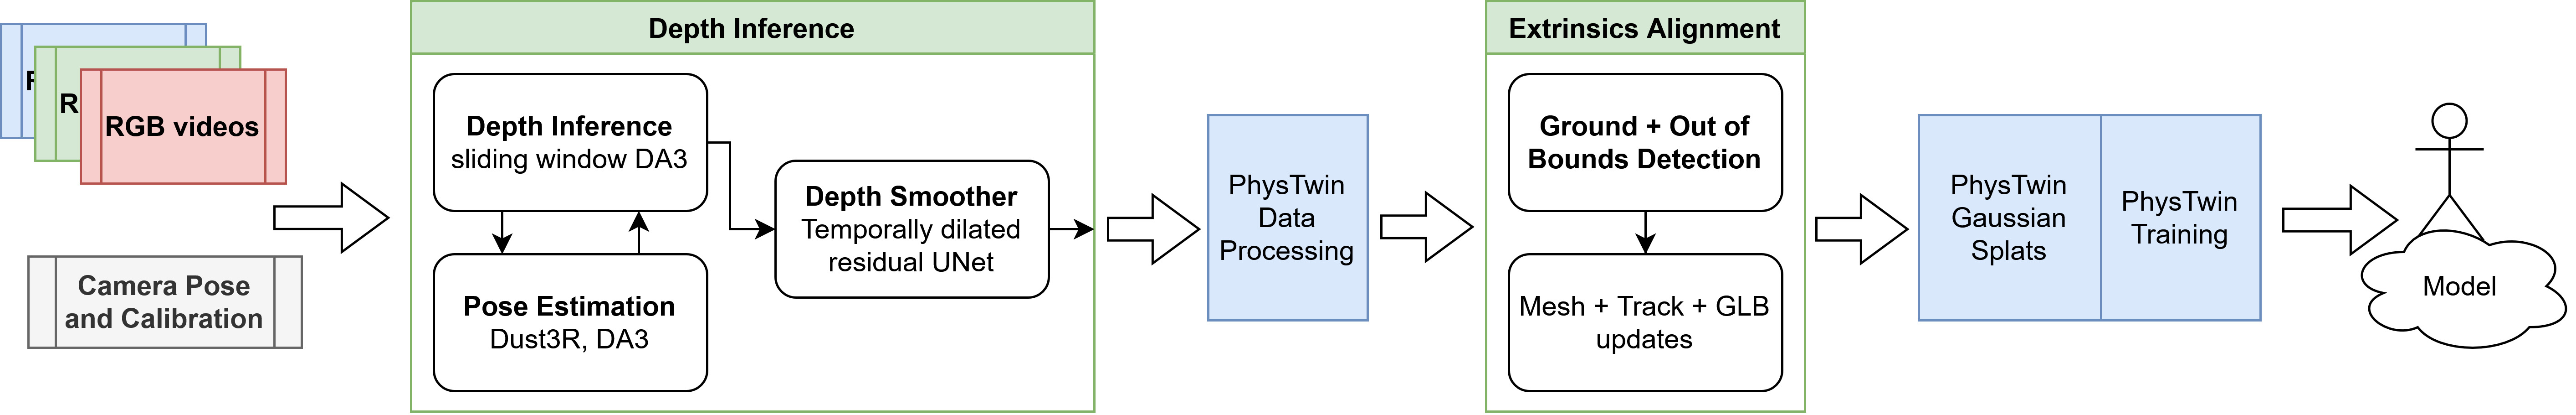
\includegraphics[width = \textwidth]{Images/pipeline_diagram_v2}
        \caption{The DIPhysTwin pipeline: camera calibration and pose estimation feed depth
        inference, whose smoothed depth maps drive the modified PhysTwin stages.}
        \label{fig:pipeline}
    \end{center}
\end{figure}

\section{Data Collection}
\label{sec:design-data}

Three datasets are used. The first is the data released with PhysTwin \parencite{phystwin}, captured
with a depth sensor; the second was collected for this project with a looser protocol, and the third with a stricter one. The first set is used to verify that the pipeline can reproduce PhysTwin's results, while the second and third sets are used to evaluate the pipeline's robustness. Table~\ref{tab:phystwin-data} summarises the released data.

\begin{table}[H]
	\caption{The data released with PhysTwin \parencite{phystwin}, summarised from the dataset
	description. The sensor depth gives this dataset a depth reference, as does the stricter
	self-collected set.}
	\label{tab:phystwin-data}
	\begin{center}
		\begin{tabular}{@{}p{3.6cm}p{10.4cm}@{}}
			\toprule
			Property & Released data \\
			\midrule
			Scenarios & 22 recorded interaction scenarios \\
			Object types & Ropes, stuffed animals, cloth, delivery packages \\
			Interactions & Quick lifting, stretching, pushing and squeezing, with one or both hands \\
			Video length & 1--10 seconds per interaction \\
			Capture rig & Three RealSense D455 RGBD cameras \\
			Annotations & 9 manually annotated ground-truth tracking points per video \\
			Split & 7:3 train/test per scenario; only the training split constructs the twin \\
			\bottomrule
		\end{tabular}
	\end{center}
\end{table}

The second self-collected set contains roughly eight laboratory interactions. The objects span soft
materials, such as a mat, stuffed animals and a plush sloth, and hard ones, such as a T-shirt and
several bottles. Intrinsics and extrinsics were deliberately not measured, because the cameras
differed from one another and the pipeline was expected to infer them. Figure~\ref{fig:irl-data} shows examples from both protocols. Data was collected with weaker constraints (two phones and a DJI action camera), rolling shutters, automatic exposure and focus, and no manual alignment of start times. This set exposed the capture
problems discussed in Chapter~\ref{cha:evaluation}.

The third set follows a stricter protocol and contains roughly thirty sessionscovering cloth, mats, bottles, mugs and stuffed animals. Three Intel RealSense D415 cameras recorded colour and
depth together, so these sessions carry a depth reference; the intrinsics and extrinsics were
measured manually as a reference only, since the pipeline used inferred poses; start times were aligned in software. Chapter~\ref{cha:discussion} treats
these properties as a source of error.

\begin{figure}[H]
	\begin{center}
		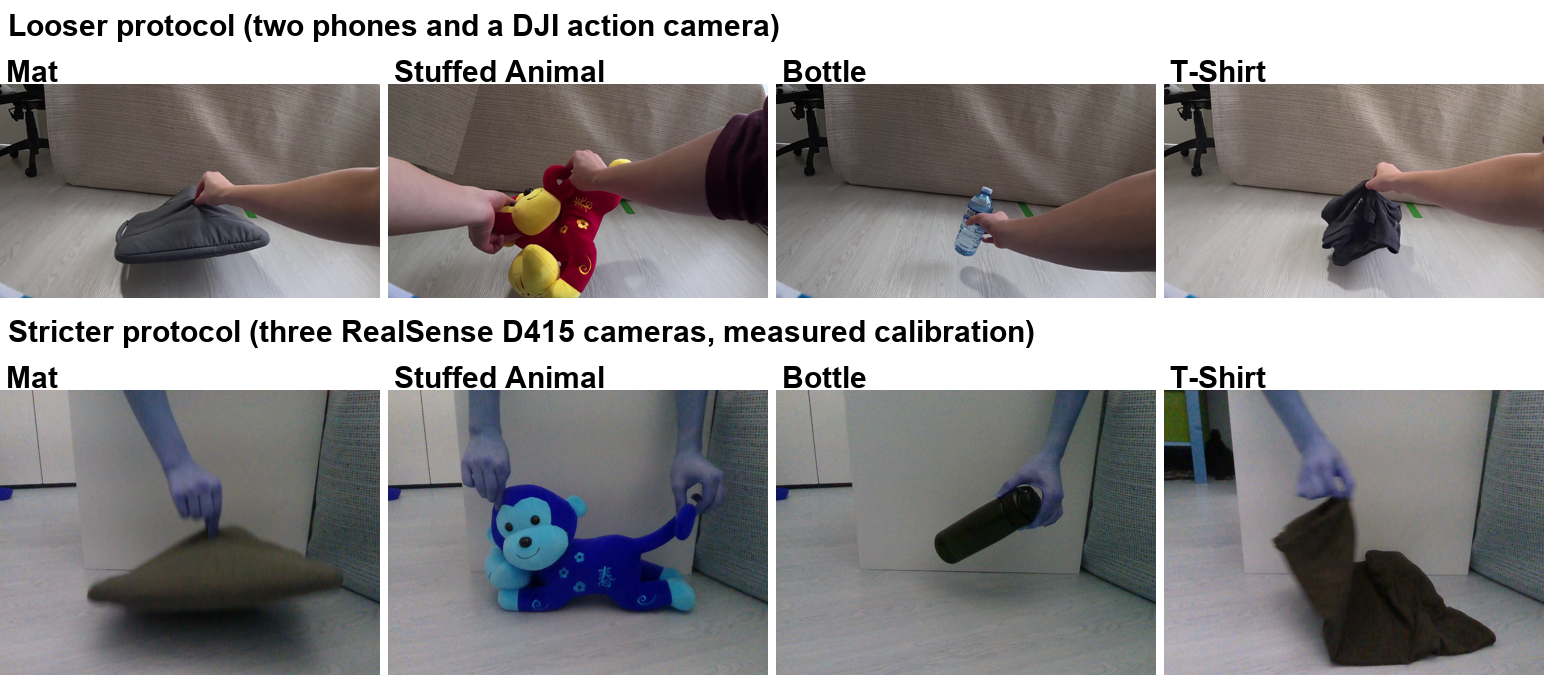
\includegraphics[width = \textwidth]{Images/irl_data}
		\caption{Example frames from the self-collected sessions: the same object categories
		captured under the looser protocol (top) and the stricter protocol (bottom).}
		\label{fig:irl-data}
	\end{center}
\end{figure}

\section{Pose Estimation and Extrinsics Alignment}
\label{sec:design-pose}

Pose estimation is a separate stage: \textcite{dust3r} builds pairwise 3D correspondences that align
much better, with a heuristic for metric scale (scaling the camera separation to $1\,\mathrm{m}$), and DA3's own pose estimation is less accurate. The estimated parameters feed data processing and alignment.

\section{Depth Inference}
\label{sec:design-depth}

Depth is estimated with \textcite{da3}, which produces non-metric but geometrically consistent views
given several camera poses. Those poses may describe a dynamic scene, or cameras positioned around a
static one.

In the inference configuration used here, depth varies between time steps and boundaries are
inconsistent. This weakens the reconstruction and adds noise to the training data. To improve
consistency, the pipeline duplicates views from stationary cameras and presents them as a dynamic
sequence, a ``fake'' sliding window. This helps over a limited number of frames. Larger windows make the Umeyama
alignment \parencite{umeyama1991} singular, so this procedure does not adapt reliably to the
sequences used here. An attempt to adapt the full model to accept multiple poses produced worse
results and was abandoned.

\label{sec:design-alignment}

Depth and pose estimation leave the scene in an arbitrary frame: the floor can be tilted, or the object can sit below or above it, but the simulator needs the ground at $z = 0$. 

The current stage back-projects the depth maps into world coordinates and fits the dominant plane
with RANSAC. The fitted plane is rotated onto $z=0$, and the same rigid
transform is applied to camera poses, tracked points and meshes so that everything stays in one
frame. The alignment script takes the first fitted
plane as the floor without checking it, and leaves a downward-pointing normal as it is.

This gives the simulator a ground plane at $z=0$. Supported objects were no longer over-stiff
once ground contact was represented.

\section{Segmentation, Shape Prior and Dense Tracking}
\label{sec:design-tracking}

Segmentation uses a promptable model \parencite{sam}. More descriptive object names produce better
masks, but some sessions still need manual intervention. Two failures were then addressed
downstream:

\begin{itemize}
	\item \textbf{Split masks.} Occlusion by the controller can break the mask into disjoint regions,
	      which defeats dense tracking. Morphological operations first rejoin them.
	\item \textbf{Non-watertight meshes.} The as-rigid-as-possible shape prior alignment
	      \parencite{arap} fails on the meshes these reconstructions produce. The fallback applies the
	      average translation of the tracked points.
\end{itemize}

\section{Implementation and Robustness Fixes}
\label{sec:design-implementation}

Several fixes cut across stages; Figure~\ref{fig:pipeline-fixes} marks where they apply.

\begin{figure}[H]
    \begin{center}
        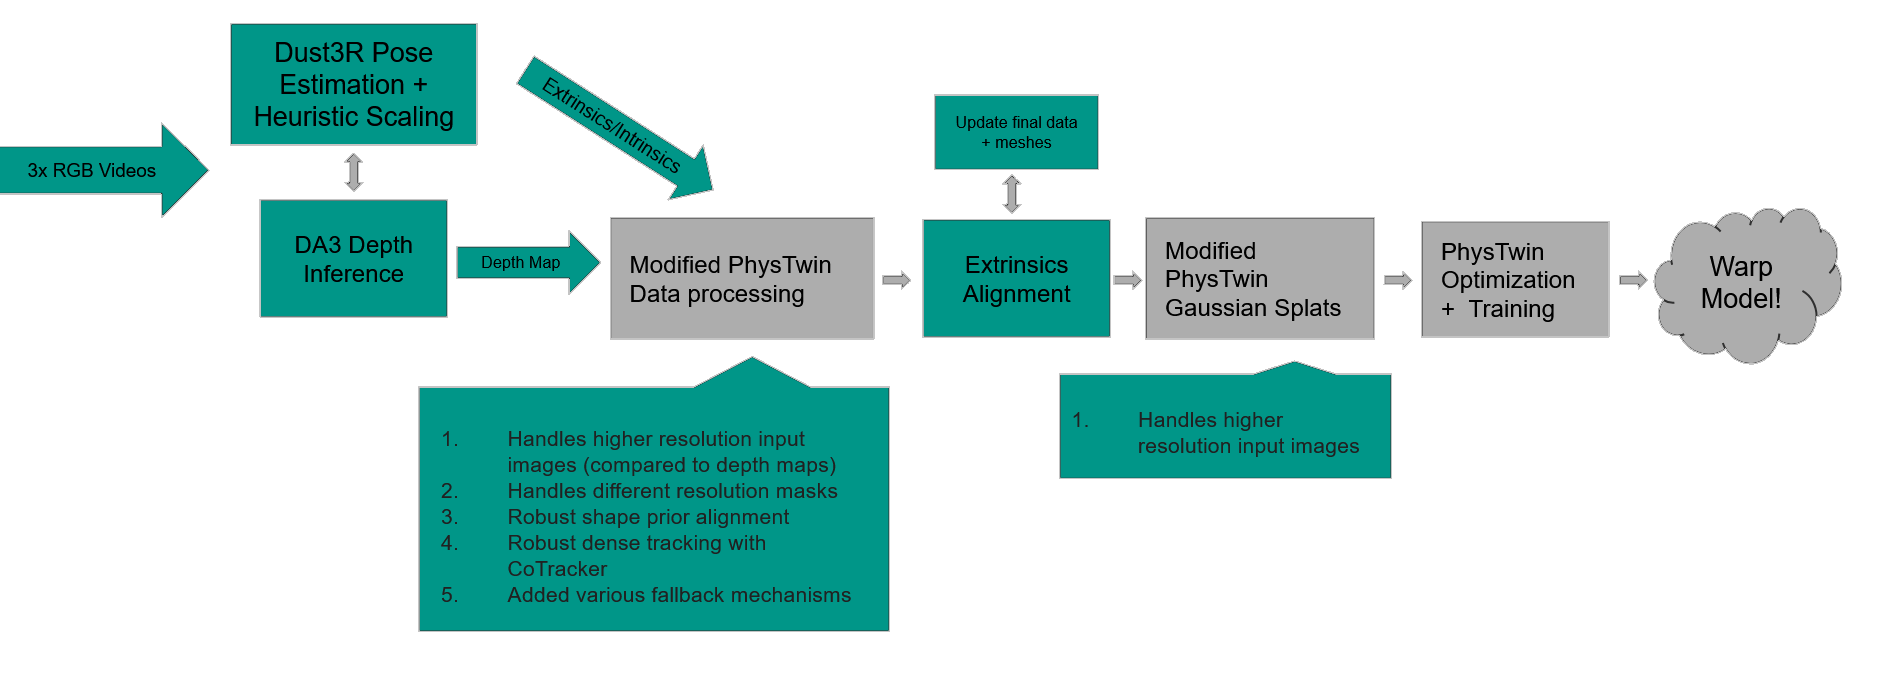
\includegraphics[width = \textwidth]{Images/pipeline_v2}		\caption{The DIPhysTwin stages with the robustness fixes marked.}
        \label{fig:pipeline-fixes}
    \end{center}
\end{figure}

\begin{itemize}
	\item \textbf{Flexible resolutions.} Hardcoded image, video and depth resolutions were
	      incompatible with the collected data, which records video at 1080p while depth maps are far
	      smaller at $280 \times 504$, and with components that prefer higher resolution. Video, depth
	      maps and masks now take independent resolutions, converted explicitly.
	\item \textbf{Idempotency.} Repeated runs produced different results, because resolution changes
	      and intrinsics were applied more than once, misaligning objects and spoiling the gaussian
	      data. Repeated runs now agree.
	\item \textbf{Fallbacks.} Where a stage can fail outright, the pipeline continues rather than
	      stopping, as in the shape prior alignment described above.
	\item \textbf{Assumptions removed.} The pipeline assumed particular position ranges within the
	      frame and a particular attachment for the controller point. Both have been generalised.
\end{itemize}
 
\chapter{Temporal Depth Smoother}
\label{cha:smoother}

A learned post-processing stage between depth inference and data processing removes temporal
flicker from inferred depth.

\section{Motivation}
\label{sec:smoother-motivation}

Depth inference (Chapter~\ref{cha:system-design}) runs a geometry model per frame on ``fake''
sliding-window input. Its depth is temporally unstable. Surfaces that do not move change depth from
one frame to the next, and the object--background and object--controller boundaries shift, so the
silhouette moves while the object itself is still. Since 2D correspondences are lifted into 3D with
these values, that jitter reaches the tracked points, the reconstruction, and the warp model.

Video depth models such as \textcite{vda} are smooth, but they are geometrically weak and monocular,
so they do not suit a multi-camera capture (see the results comparison in Table~\ref{tab:app-vid-variants}, Appendix~\ref{app:results}). Earlier stabilisation work either couples to a specific
depth backbone \parencite{nvds,nvdsp} or assumes labelled sensor ground truth
\parencite{stabledpt,li2023consistent}. The stage described here has to meet a narrower requirement:
it must apply to any flickering depth sequence, need no ground truth, and work across views.

\section{Learning a Residual Correction}
\label{sec:smoother-idea}

The two model families fail in opposite places: the geometry model has good \emph{spatial}
structure, and the video model has good \emph{temporal} structure. Depth and RGB are encoded into a
latent space and decoded into a smooth prediction, which is scored by temporal penalties taken from
the video model and geometric penalties taken from the geometry model.

Rather than predict a depth map, the network predicts a \emph{residual} that is added to the geometry
model's prediction. The video model serves as a motion oracle, not a depth reference: its values are
relative, so no metric scale is inherited from it.

\section{Architecture}
\label{sec:smoother-architecture}

\begin{figure}[H]
	\begin{center}
		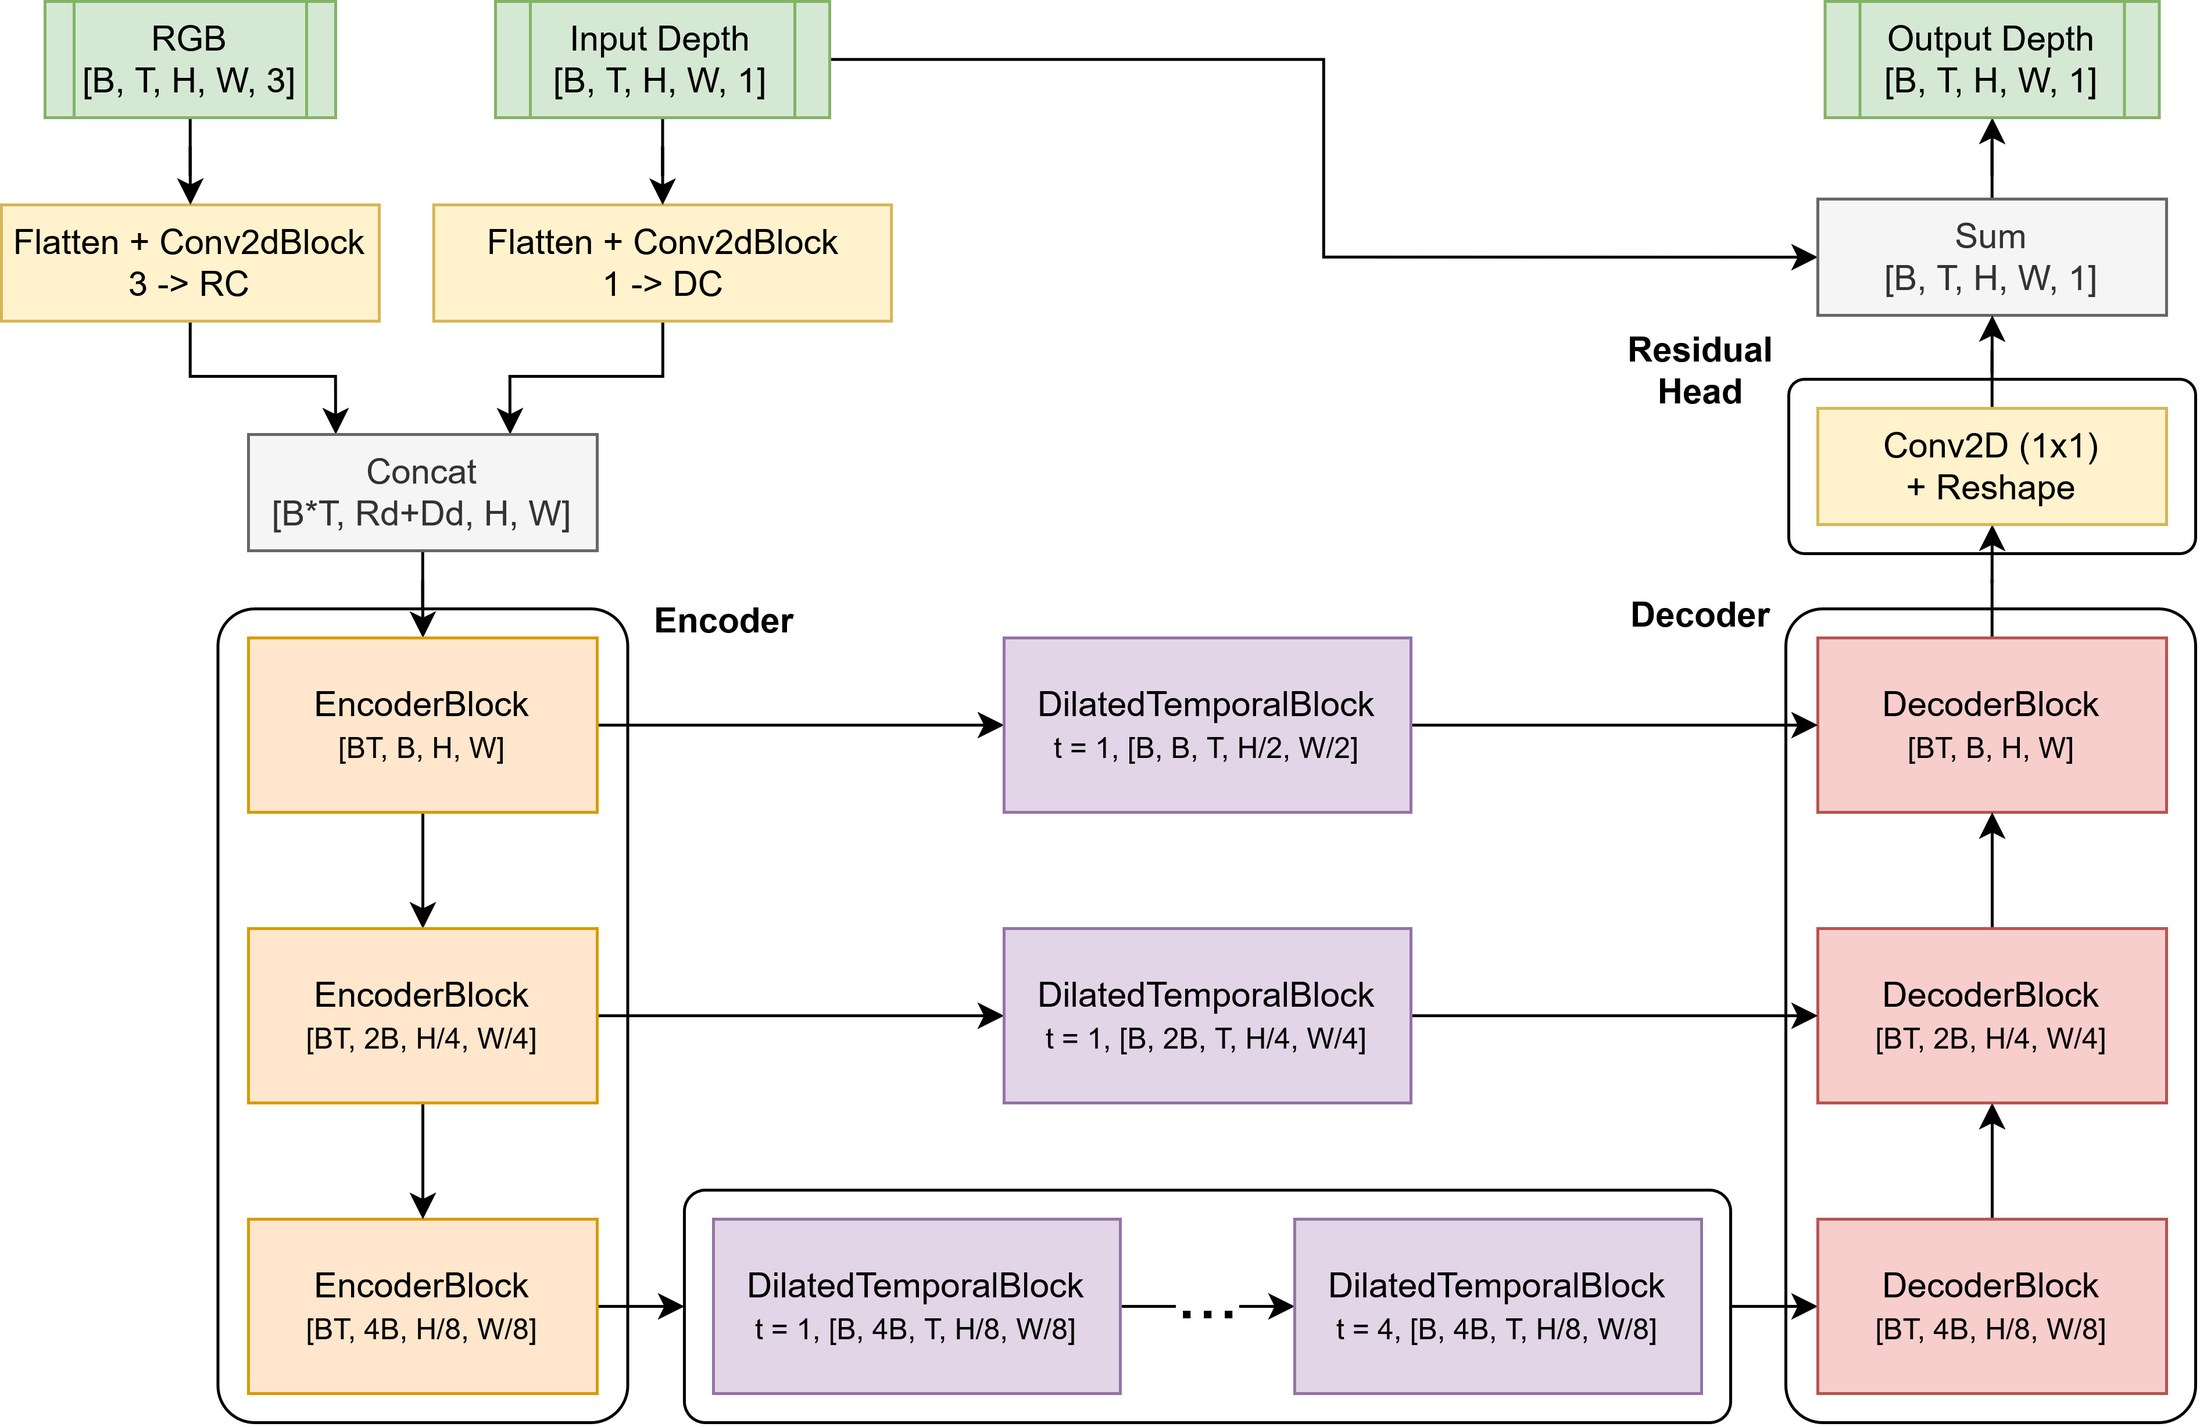
\includegraphics[width = 0.9\textwidth]{Images/smoother_architecture}
		\caption{The temporally-dilated residual U-Net.}
		\label{fig:smoother-architecture}
	\end{center}
\end{figure}

The network has to learn and preserve structure from the geometry model, absorb temporal consistency
from the video model, and correct each frame using both depth maps and the RGB image. A diffusion-
or DPT-style backbone was considered and rejected, because it was deemed overkill and potentially too expensive. The chosen design is a small 4.7-million-parameter \textbf{temporally-dilated residual U-Net}.
Spatial structure is preserved across scales, and temporal dilation gives each frame context from
several time offsets without processing the whole clip. Its size is limited by the training compute
available.

The U-Net is assembled from four blocks (Figure~\ref{fig:smoother-blocks}). The per-frame 2D block,
\texttt{Conv2dBlock}, is two $3\times3$ convolutions, each followed by GroupNorm and ReLU. An
\texttt{EncoderBlock} runs one of these and taps the skip connection before a strided $2\times2$
convolution halves the resolution. A \texttt{DecoderBlock} doubles the resolution with a transposed
convolution, concatenates the matching skip and refines the result with a \texttt{Conv2dBlock}; a
learned upsample is used because bilinear upsampling produced smearing and edge artefacts. The
\texttt{DilatedTemporalBlock} is a single $3\times3\times3$ convolution, dilated only in time, with
GroupNorm, ReLU and a residual connection. Stacking dilations $1, 2, 4, 8$ at the bottleneck gives
each output frame a receptive field of $\pm15$ frames; shallower levels use dilation 1.

\begin{figure}[H]
	\begin{center}
		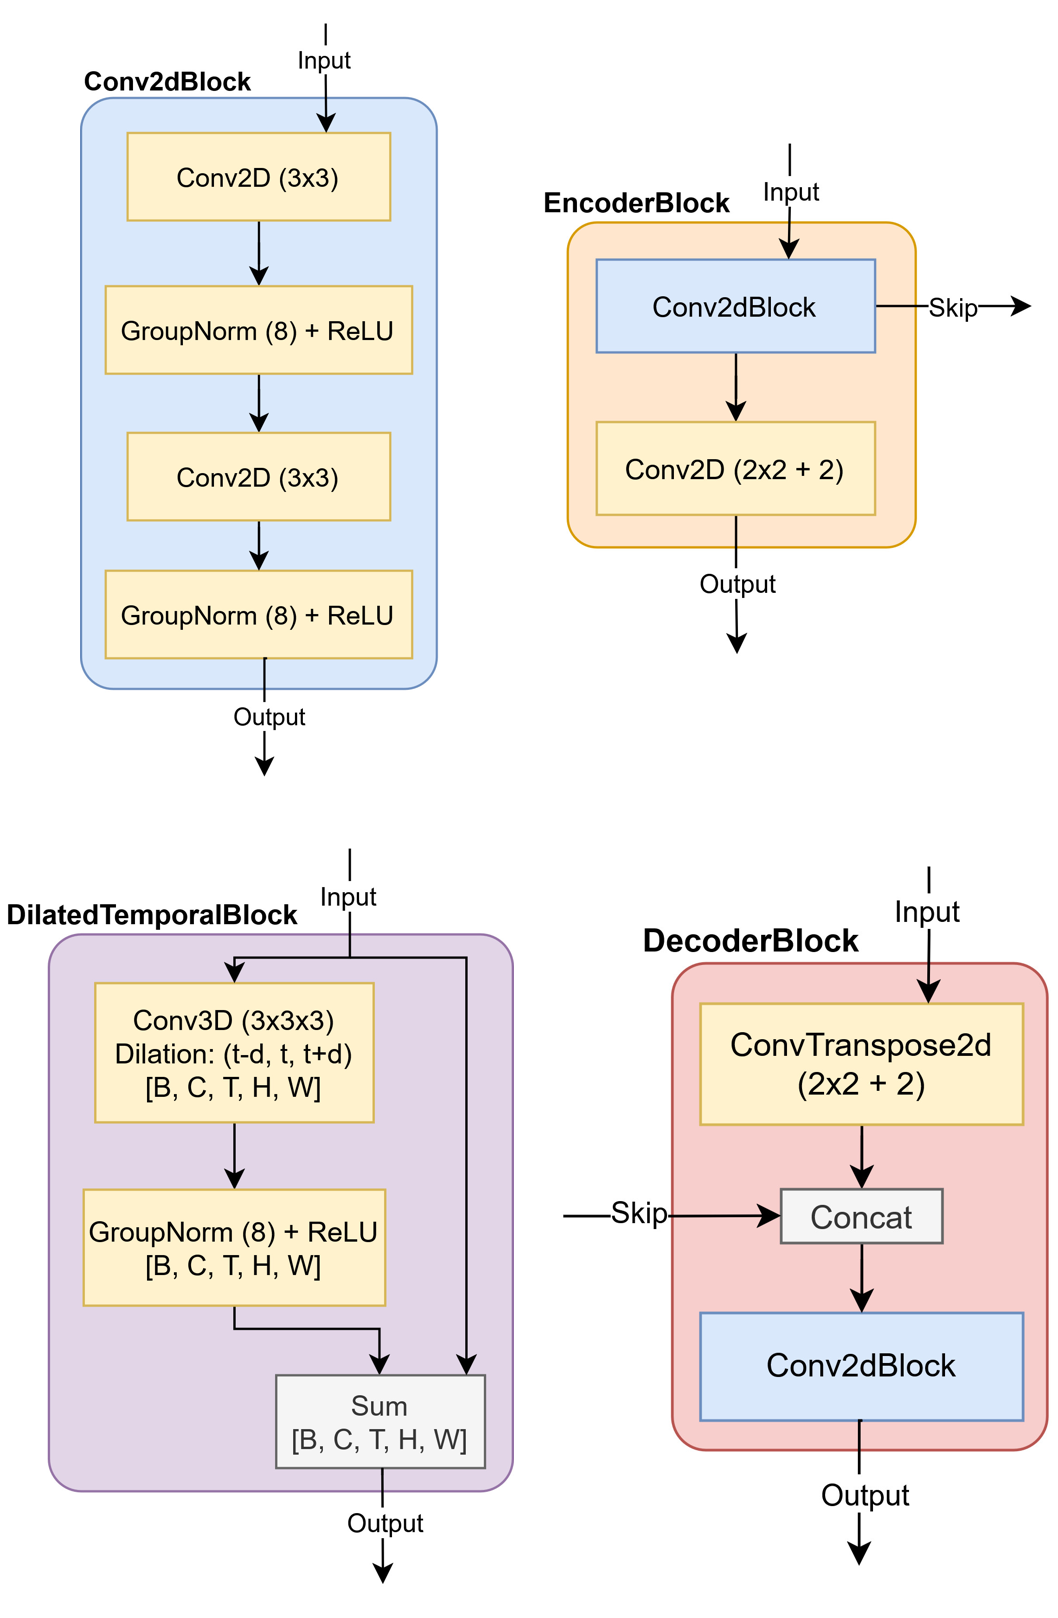
\includegraphics[width = 0.8\textwidth]{Images/block_grid}
		\caption{The four building blocks of the smoother, drawn to a common scale:
		(a)~\texttt{Conv2dBlock}, (b)~\texttt{EncoderBlock}, (c)~\texttt{DilatedTemporalBlock} and
		(d)~\texttt{DecoderBlock}, which reinserts the skip connection that the encoder taps.}
		\label{fig:smoother-blocks}
	\end{center}
\end{figure}


\section{Loss Functions}
\label{sec:smoother-losses}

The objective combines fidelity, temporal gradient matching (TGM), temporal total variation (TV),
and two geometric penalties: edge sharpness and spatial-gradient matching. 

Let $D^s$, $D^0$ and $D^v$ denote the smoothed output, raw DA3 depth and aligned VDA depth. For
frame skip $k$, define
\[
    \Delta_k D_{b,t,x}=D_{b,t+k,x}-D_{b,t,x},\qquad
    \Delta_k^2D_{b,t,x}=D_{b,t+2k,x}-2D_{b,t+k,x}+D_{b,t,x}.
\]
Here $b$ indexes a clip, $t$ a frame and $x$ a pixel. Angle brackets denote a mean over valid
clips, frame indices and pixels. Denominators are clamped below by $\epsilon=10^{-6}$. The equations follow the implementation.

\paragraph{Temporal gradient matching loss.}
\label{sec:smoother-tgm}

For each span $k$, TGM matches temporal depth differences to VDA. The VDA values provide a motion
signal, not a depth target. Each span is normalised by the discrepancy between raw DA3 and VDA:
\[
    B_{\mathrm{tgm}}^{(k)}
      =\max\!\left(\left\langle\left|\Delta_kD^0-\Delta_kD^v\right|\right\rangle,\epsilon\right),
    \qquad
    \mathcal{L}_{\mathrm{tgm}}^{(k)}
      =\frac{\left\langle\left|\Delta_kD^s-\Delta_kD^v\right|\right\rangle}
                  {B_{\mathrm{tgm}}^{(k)}}.
\]
The implementation combines $k=1,2,3$ as
\[
    \mathcal{L}_{\mathrm{tgm}}
      =\mathcal{L}_{\mathrm{tgm}}^{(1)}
       +0.25\,\mathcal{L}_{\mathrm{tgm}}^{(2)}
       +0.07\,\mathcal{L}_{\mathrm{tgm}}^{(3)}.
\]
Larger skips capture slower oscillations; their weights are code defaults and have not been
systematically tuned.


\paragraph{Temporal total variation loss.}
\label{sec:smoother-tv}

TV penalises the output's second temporal difference. VDA acceleration gates the penalty, reducing
it where the motion oracle reports acceleration. For each span,
\[
    w_{b,t,x}^{(k)}
      =\exp\!\left(-10\left|\Delta_k^2D^v_{b,t,x}\right|\right),
    \qquad
    B_{\mathrm{tv}}^{(k)}
      =\max\!\left(\left\langle\left|\Delta_k^2D^0\right|w^{(k)}\right\rangle,\epsilon\right),
\]
\[
    \mathcal{L}_{\mathrm{tv}}^{(k)}
      =\frac{\left\langle\left|\Delta_k^2D^s\right|w^{(k)}\right\rangle}
                  {B_{\mathrm{tv}}^{(k)}},
    \qquad
    \mathcal{L}_{\mathrm{tv}}
      =\mathcal{L}_{\mathrm{tv}}^{(1)}+0.25\,\mathcal{L}_{\mathrm{tv}}^{(2)}.
\]
The exponential constant and span weights come from the implementation and were not tuned.


\paragraph{Fidelity loss.}
\label{sec:smoother-fidelity}

Fidelity keeps the output close to DA3 in a shared, clip-level scale. Let $m_{b,x}=\operatorname{median}_tD^0_{b,t,x}$,
$t_b=\operatorname{median}_x m_{b,x}$ and
$s_b=\max(\operatorname{mean}_x|m_{b,x}-t_b|,\epsilon)$. The aligned depth is
$A_b(D)=(D-t_b)/s_b$. For the VDA gate, let
$\mu_v=\langle|\Delta_1D^v|\rangle+\epsilon$ and $\gamma=0.25$:
\[
    g_{b,0,x}=1,\qquad
    g_{b,t,x}=\gamma+(1-\gamma)
       \exp\!\left(-\frac{|\Delta_1D^v_{b,t-1,x}|}{\mu_v}\right),\quad t>0,
\]
\[
    B_{\mathrm{fid}}=\max\!\left(\operatorname{std}(A(D^0)),\epsilon\right),
    \qquad
    \mathcal{L}_{\mathrm{fid}}
      =\frac{\left\langle g\,|A(D^s)-A(D^0)|\right\rangle}{B_{\mathrm{fid}}}.
\]
The gate is strongest in temporally stable regions and relaxes toward $0.25$ where VDA reports
motion. Its scale and location statistics are computed from DA3, not VDA.


\paragraph{Geometric loss.}
\label{sec:smoother-geometric}

The implementation has two spatial penalties. Define forward finite differences by
$\nabla_xD_{b,t,i,j}=D_{b,t,i,j+1}-D_{b,t,i,j}$ and
$\nabla_yD_{b,t,i,j}=D_{b,t,i+1,j}-D_{b,t,i,j}$, padding the last column and row with zero.
The edge-sharpness penalty uses Sobel magnitudes $G(I)$ of grayscale RGB and $G(D^v)$ of VDA
depth, each divided by its per-clip 95th percentile. It keeps pixels identified as edges in both
signals and penalises smoothed edges below $0.8$ of the VDA edge magnitude:
\[
    M=\mathbf{1}[\widetilde G(I)>0.6]\,\mathbf{1}[\widetilde G(D^v)>0.6],\qquad
    \mathcal{L}_{\mathrm{edge}}
      =\frac{\operatorname{mean}_{M=1}
             [\,0.8\widetilde G(D^v)-\widetilde G(D^s)\,]_+}
             {\max\!\left(\operatorname{mean}_{M=1}\widetilde G(D^v),\epsilon\right)}.
\]
Here $[q]_+=\max(q,0)$; an empty mask gives zero numerator. The second penalty compares forward
finite-difference gradients of smoothed and raw DA3 depth, weighted by VDA Sobel magnitude. With
$W=\max(0.1,G(D^v)/(\operatorname{mean}_{t,x}G(D^v)+\epsilon))$,
\[
    \mathcal{L}_{\mathrm{grad}}
      =\frac{\frac12\sum_{a\in\{x,y\}}\left\langle W\,
             |\nabla_aD^s-\nabla_aD^0|\right\rangle}
             {\max\!\left(\frac12\sum_{a\in\{x,y\}}\left\langle W|\nabla_aD^0|\right\rangle,
             \epsilon\right)}.
\]
Both spatial terms are baseline-normalised in the implementation. Their individual effects have
not been isolated in the evaluation.


\paragraph{Combined objective.}
\label{sec:smoother-combined}

The weighted objective is
\[
    \mathcal{L}
      =\lambda_{\mathrm{fid}}\mathcal{L}_{\mathrm{fid}}
       +\lambda_{\mathrm{tgm}}\mathcal{L}_{\mathrm{tgm}}
       +\lambda_{\mathrm{tv}}\mathcal{L}_{\mathrm{tv}}
       +\lambda_{\mathrm{edge}}\mathcal{L}_{\mathrm{edge}}
       +\lambda_{\mathrm{grad}}\mathcal{L}_{\mathrm{grad}}.
\]
The training configuration gives $\lambda_{\mathrm{fid}}=1.3$, $\lambda_{\mathrm{tgm}}=0.8$,
$\lambda_{\mathrm{tv}}=0.8$, $\lambda_{\mathrm{edge}}=0.05$ and
$\lambda_{\mathrm{grad}}=0.04$. The span weights are listed in Appendix~\ref{app:hyperparameters}. These settings remain untuned.


\section{Training}
\label{sec:smoother-training}

The training run uses 162 complete clip-camera inputs and saves a
best-model checkpoint. The deterministic split is by clip, so frames from a validation clip do not
enter training. Table~\ref{tab:smoother-training} records the training configuration.

\begin{table}[H]
    \caption{Temporal smoother training configuration.}
    \label{tab:smoother-training}
    \begin{center}
        \begin{tabular}{@{}p{3.6cm}p{10.4cm}@{}}
            \toprule
            Setting & Recorded value \\
            \midrule
            Complete clips & 162 clip-camera inputs; 130 train and 32 validation (80:20, seed 42, split by clip) \\
            Training samples & 1,842 windows; length 16 frames, stride 8 \\
            Validation samples & 264 windows; length 16 frames, stride 16 \\
            Input size & $226\times334$ pixels; RGB and depth are resized \\
            Batch and workers & Batch size 2; 2 data-loader workers \\
            Optimiser & Adam; weight decay $10^{-4}$ \\
            Learning rate & $3\times10^{-3}$; ReduceLROnPlateau, factor $0.5$, patience 5 \\
            Duration & 50 epochs; checkpoints saved for each epoch \\
            Precision & CUDA autocast with bfloat16 enabled \\
            Loss weights and temporal spans & See Table~\ref{tab:app-lossweights} (Appendix~\ref{app:hyperparameters}) \\

            Augmentation and hardware & No augmentation in the loader; NVIDIA GeForce RTX 3060 \\
            \bottomrule
        \end{tabular}
    \end{center}
\end{table}

Training ran on a single NVIDIA GeForce RTX 3060. The loader resizes and normalises inputs but
applies no augmentation.


\section{Inference}
\label{sec:smoother-inference}

Inference follows the video model. Clips are processed in overlapping chunks, which provides
temporal context without holding an entire sequence in memory; the chunks are blended with the
weighted window of Figure~\ref{fig:smoother-inference}. Resolutions are arbitrary with minimal
padding, and depth maps are never resized, since resizing would destroy the sub-pixel frame-to-frame
consistency the stage exists to produce.

\begin{figure}[H]
	\begin{center}
		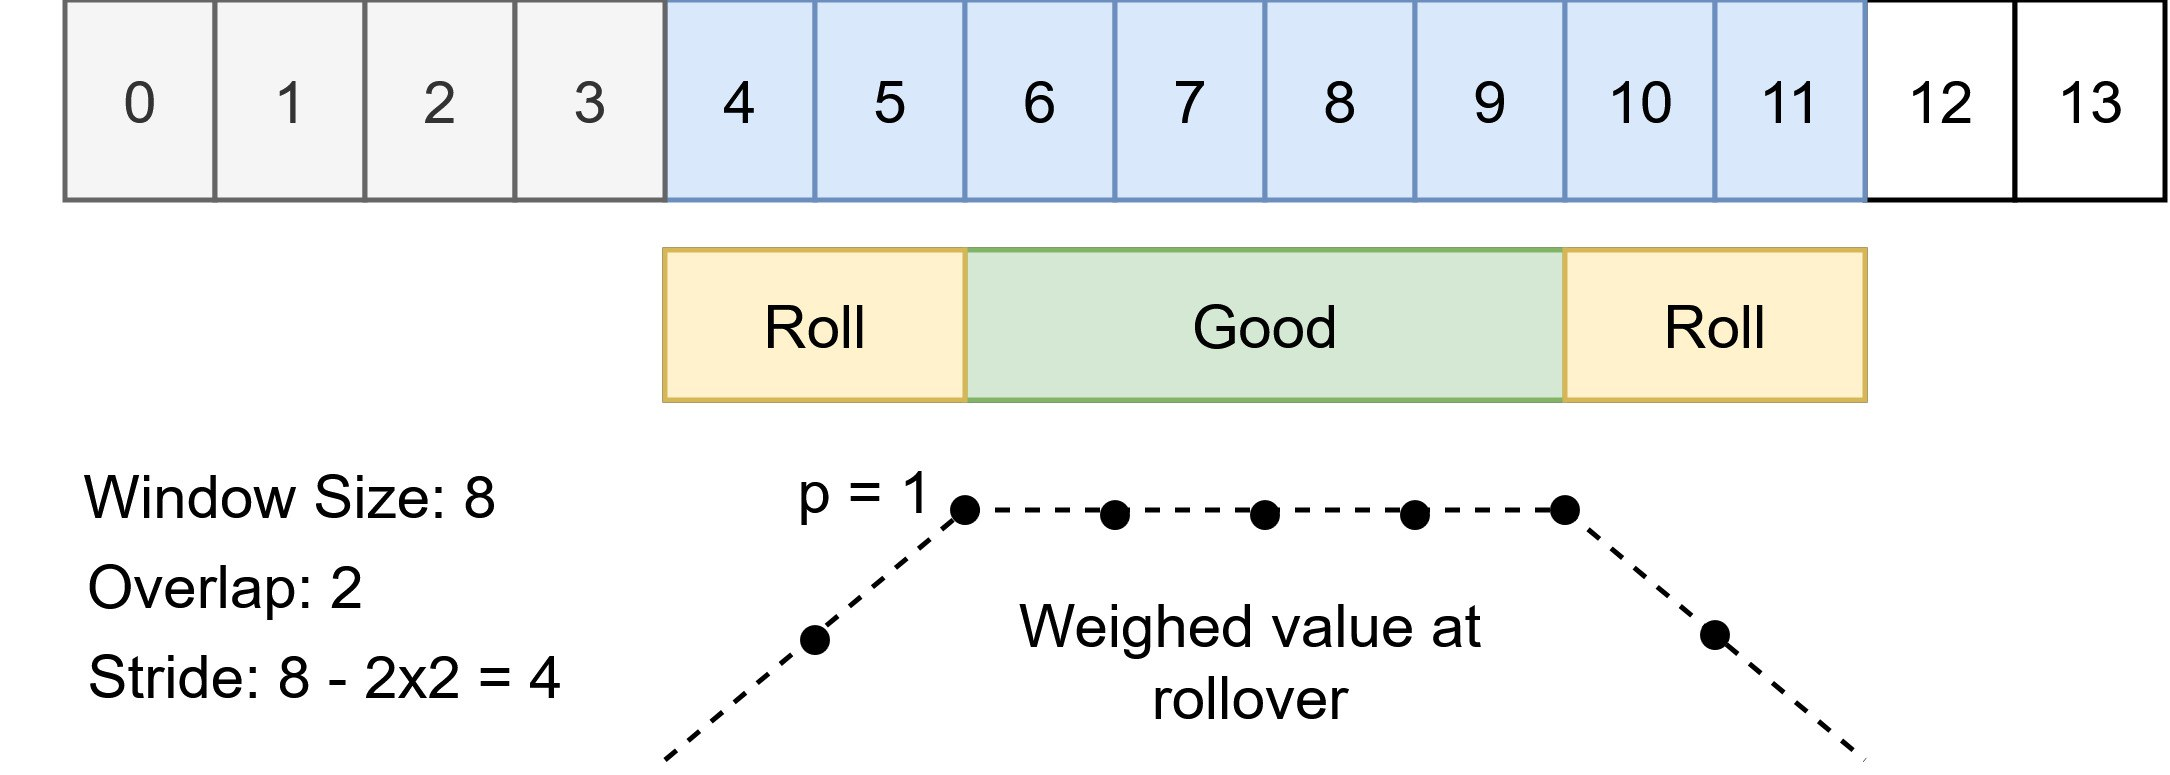
\includegraphics[width = \textwidth]{Images/smoother_inference}
		\caption{Weighted sliding-window inference. Overlapping chunks are blended into one output
		sequence.}
		\label{fig:smoother-inference}
	\end{center}
\end{figure}

Figure~\ref{fig:smoother-beforeafter} shows four frames, two each from a mat lift and a sloth
stretch, before and after smoothing with the best saved model. Consecutive-frame comparisons over
five sequences are shown in Figure~\ref{fig:eval-depth-cases} (Chapter~\ref{cha:evaluation});
full recorded clips are listed in Appendix~\ref{app:results}.

\begin{figure}[H]
	\begin{center}
		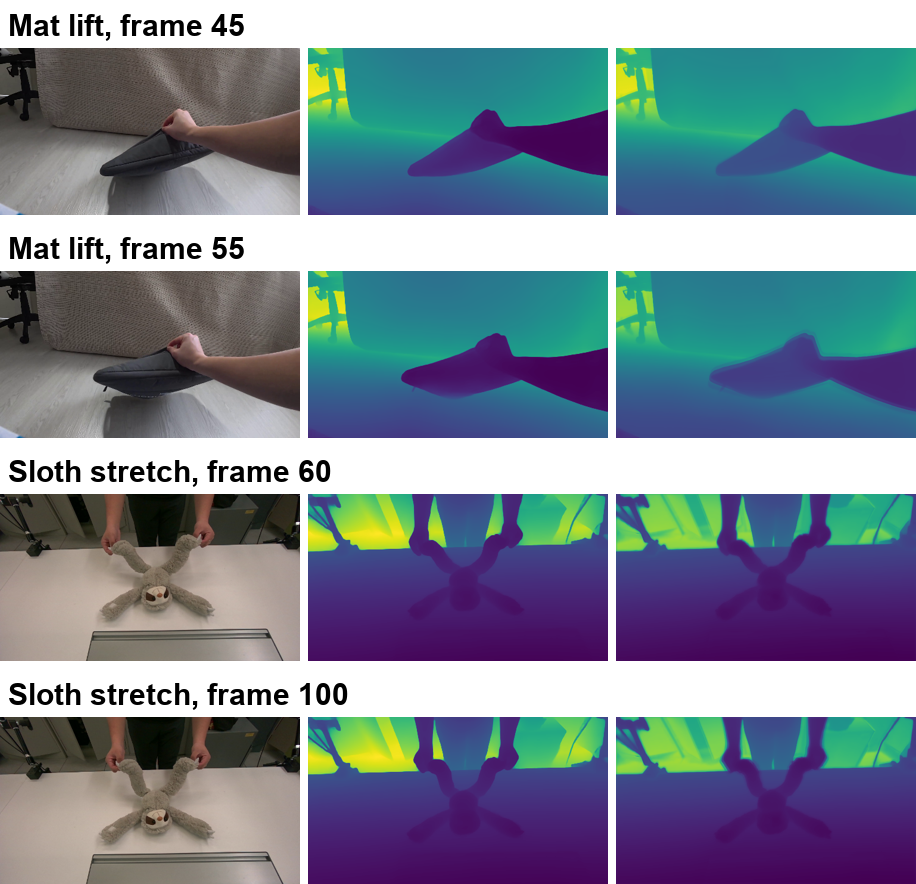
\includegraphics[width = \textwidth]{Images/smoother_beforeafter}
		\caption{RGB input, raw DA3 depth and smoothed depth for four frames of a mat-lift and a
		sloth-stretch sequence.}
		\label{fig:smoother-beforeafter}
	\end{center}
\end{figure}


\section{Properties and Limitations}
\label{sec:smoother-properties}

The stage can be reused independently of this project:

\begin{enumerate}
	\item It applies to any flickering depth map, because it predicts a correction and needs no
	      specific backbone.
	\item It requires no ground-truth depth and no labelled dataset.
	\item It handles arbitrary resolutions without resizing.
	\item It is small and fast relative to the depth model it corrects.
\end{enumerate}

Some limitations remain. Smoothing visibly blurs depth, and there is not enough evidence that the
correction targets object flicker vs stationary flicker. The hyper-parameters are untuned, and the
results depend heavily on these settings. The stage has not been validated on other depth backbones, and it is not clear how well it generalises to other domains.

\chapter{Evaluation}
\label{cha:evaluation}

This chapter reports the depth comparison and qualitative pipeline results. The looser
self-collected videos have no depth ground truth, so most measures here address stability and
geometry preservation rather than accuracy.

\section{Evaluation Setup and Datasets}
\label{sec:eval-setup}

The evaluation uses PhysTwin's released RGBD data \parencite{phystwin} and about 30 self-collected
multi-view sessions of cloth, mats, bottles, mugs and stuffed animals; an earlier batch contained
about eight sessions. The first rig used two phones and a DJI action camera, with different
intrinsics, rolling shutters, auto-exposure and autofocus. The cameras were not time-synchronised.
The later rig recorded colour and depth with three Intel RealSense D415 cameras and measured the
intrinsics and extrinsics manually as a reference, although the pipeline still infers poses; those sessions carry a metric depth reference, and the earlier
batch has none.


\section{Measuring Depth Quality Without Ground Truth}
\label{sec:eval-protocol}

A depth error can only be measured against a sensor reference. PhysTwin's released sequences and
the stricter self-collected sessions both carry sensor depth, but it is sparse and noisy relative to
the dense predictions, and the looser-protocol videos have no reference at all. The evaluation
therefore reports one relative comparison against the sensor
(Section~\ref{sec:eval-depth-sensor}), covering a single sequence, and treats the rest
qualitatively: flicker removal (Section~\ref{sec:eval-depth-cases}), tracking
(Section~\ref{sec:eval-tracking}) and the end-to-end results. Each result is only a proxy, because
smoothing can reduce flicker while flattening or blurring geometry. There are no cross-view or
warp-model scores, and no quantitative VDA or streaming-baseline comparison. End-to-end findings
below are the author's own visual judgement. No other raters scored them, and no formal rating protocol was used. No loss-term ablation
or temporal-span sweep was performed; their effects and weight sensitivity remain
unmeasured.\label{sec:eval-ablations}


\section{Depth against the sensor reference}
\label{sec:eval-depth-sensor}
\label{sec:eval-depth}

PhysTwin's released sequences carry RealSense depth, as do the stricter self-collected sessions,
which were recorded with three RealSense D415 cameras capturing colour and depth together. The
comparison below uses the released double-stretch sloth sequence: the raw inferred depth and the
smoothed depth were each compared with the sensor reference over all 192 frames of the three
cameras (\texttt{evaluation/compare\_depth.py}).
The comparison measures relative depth: Spearman rank correlation of the depth ordering, Pearson
correlation of Sobel gradient magnitudes, the ordinal error (the fraction of sampled point pairs
whose ordering is reversed), and the scale-invariant RMSE after a
least-squares scale-and-shift alignment. The sensor depth is sparse and noisy around object
boundaries, which limits all four measures.

\begin{figure}[H]
	\begin{center}
		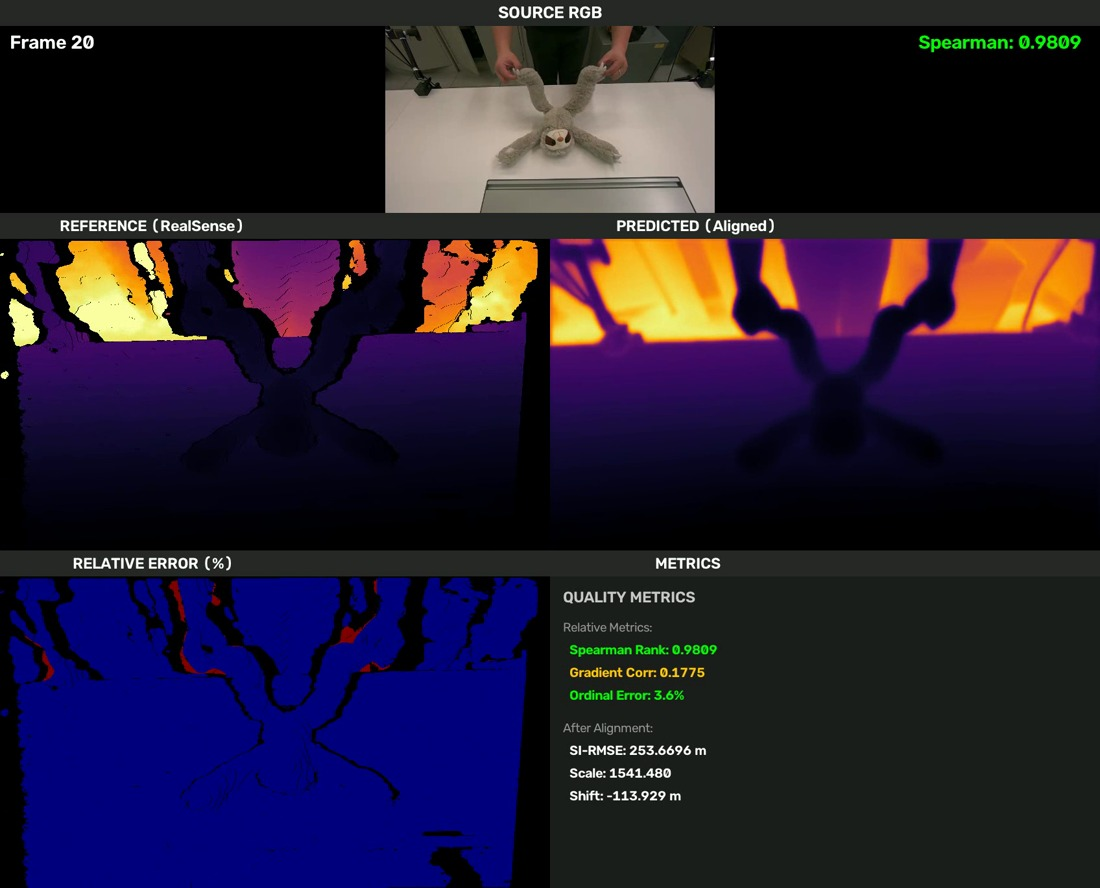
\includegraphics[width = \textwidth]{Images/depth_vs_sensor}
		\caption{One frame (20 of 192) of the sloth sequence after smoothing: source RGB, RealSense
		reference depth, aligned smoothed depth, error map and per-frame metrics.}
		\label{fig:eval-depth-sensor}
	\end{center}
\end{figure}

\begin{table}[H]
    \caption{Relative depth quality against the RealSense reference over 192 frames of the
    double-stretch sloth sequence, per camera, for the raw inferred depth (top) and the smoothed
    depth (bottom). SI-RMSE is in millimetres after scale-and-shift alignment.}
    \label{tab:eval-depth-sensor}
    \begin{center}
        \small
        \begin{tabular}{@{}llcccc@{}}
            \toprule
            Depth & Camera & Spearman $\uparrow$ & Gradient corr.\ $\uparrow$ & Ordinal error $\downarrow$ & SI-RMSE $\downarrow$ \\
            \midrule
            Raw DA3 & 0 & 0.988 & 0.117 & 3.3\% & 346 \\
                    & 1 & 0.945 & 0.115 & 6.9\% & 666 \\
                    & 2 & 0.963 & 0.090 & 4.2\% & 1495 \\
            \midrule
            Smoothed & 0 & 0.988 & 0.169 & 3.3\% & 343 \\
                     & 1 & 0.951 & 0.151 & 6.6\% & 664 \\
                     & 2 & 0.964 & 0.122 & 4.5\% & 1494 \\
            \bottomrule
        \end{tabular}
    \end{center}
\end{table}

The depth ordering is nearly perfect for both variants and few point pairs are misordered. Smoothing
leaves the ordering and the aligned error almost unchanged and raises the gradient correlation on every
camera (0.107 to 0.147 on average), so the smoothed depth still agrees with the sensor
reference. On camera 0 the per-frame ordinal error varies little (2.3--4.6\%, median 3.25\%): most
sampled pairs span large depth differences, which both variants order correctly, while the errors
concentrate on near-tie pairs within the object and at its boundary. The gradient correlation is
still modest: local depth structure remains weaker than the
sensor's, which matches the inconsistent boundaries observed in Section~\ref{sec:design-depth}. The
measurement covers one sequence and compares the inferred depth with the sensor; it does not compare
the four depth sources end to end.

\begin{figure}[H]
	\begin{center}
		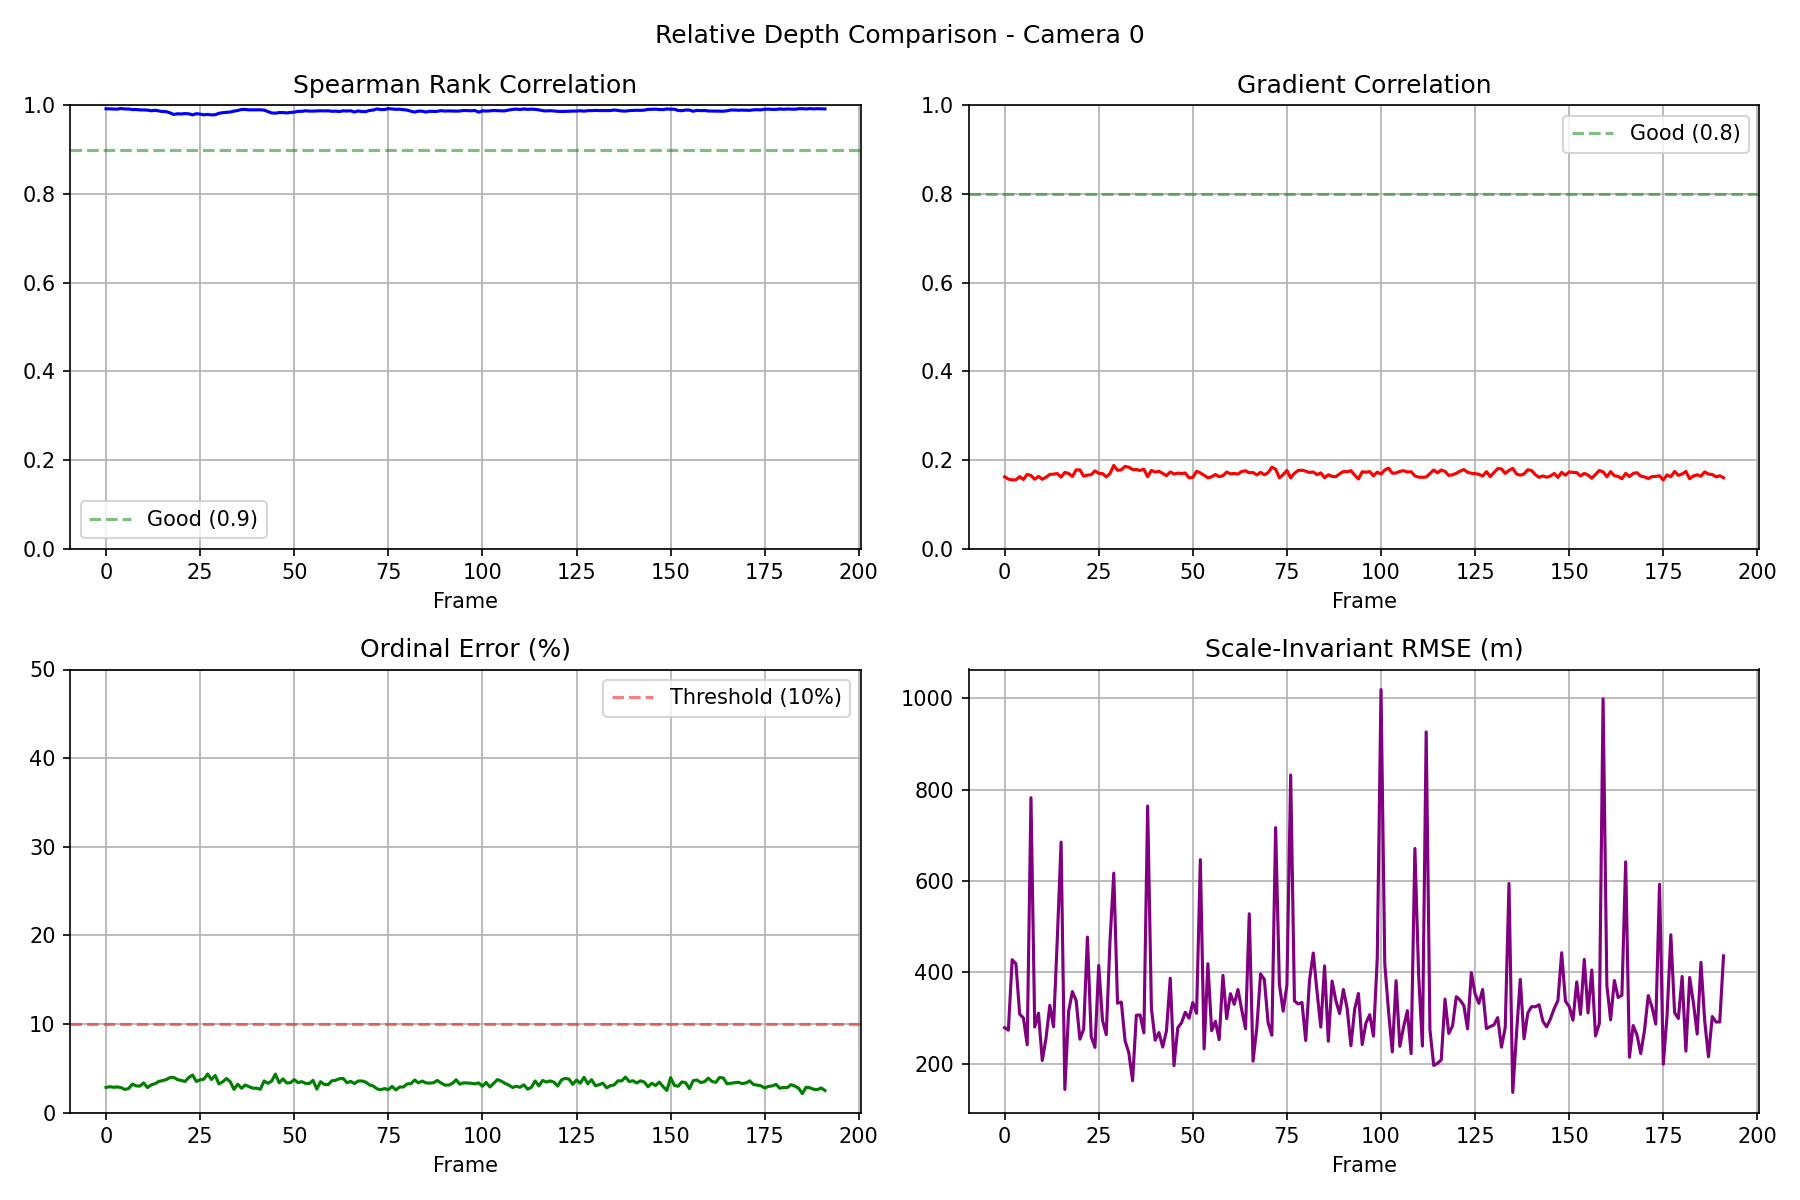
\includegraphics[width = 0.85\textwidth]{Images/depth_quality_metrics}
		\caption{Per-frame relative depth metrics for the smoothed depth, camera 0: Spearman rank
		correlation, gradient correlation, ordinal error and SI-RMSE.}
		\label{fig:eval-depth-metrics}
	\end{center}
\end{figure}

\section{Flicker removal across sequences}
\label{sec:eval-depth-cases}

Figures~\ref{fig:eval-depth-cases} and~\ref{fig:eval-depth-cases-2} show five consecutive frames
of five sequences, raw DA3 above and smoothed below, with a shared colour scale per sequence. In the
raw rows the depth of static surfaces shifts from frame to frame and the object--background boundary
moves; the smoothed rows are stable frame to frame at the cost of softer boundaries. The smoothed
rows come from the best saved model,
\texttt{best\_model\_50\_epochs\_no\_edge\_blur}. Sequences include sloth, monkey, mat, rope and
cloth; the monkey and mat rows use looser-protocol captures. Video recordings of the raw
and smoothed depth are listed in Appendix~\ref{sec:app-vid-smoother}, and pipeline replays before and
after smoothing in Appendix~\ref{sec:app-vid-smoother}.

\begin{figure}[H]
	\begin{center}
		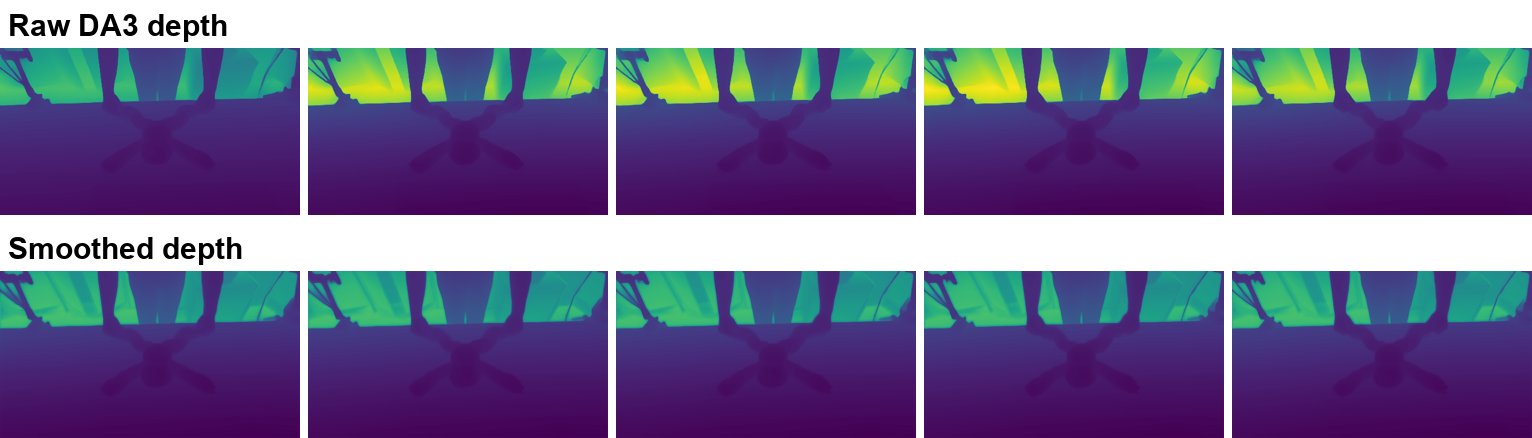
\includegraphics[width = \textwidth]{Images/depth_case_sloth}\\
		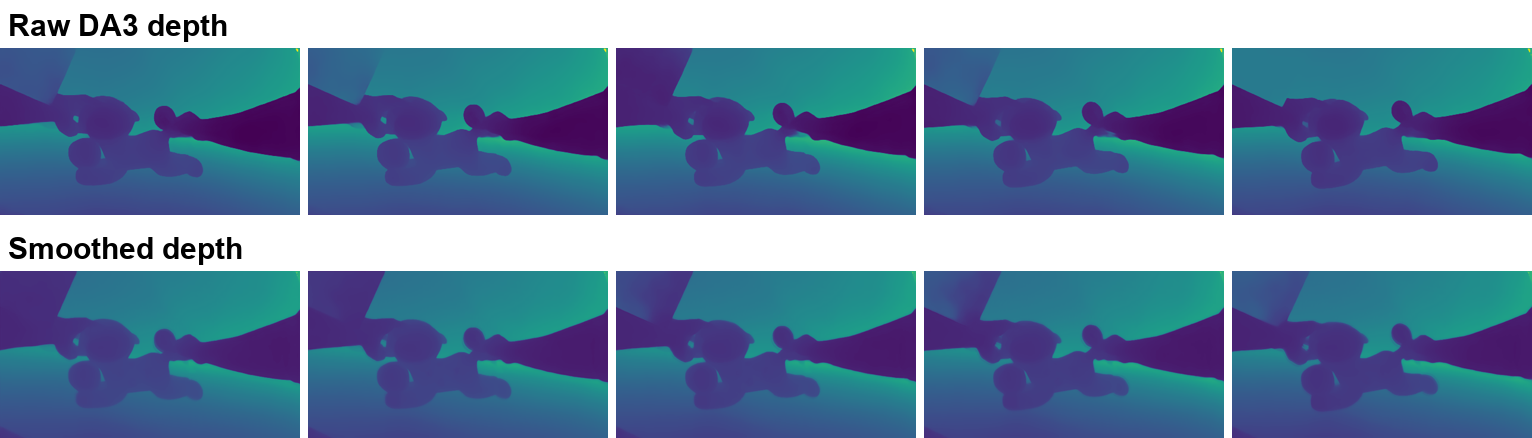
\includegraphics[width = \textwidth]{Images/depth_case_monkey}\\
		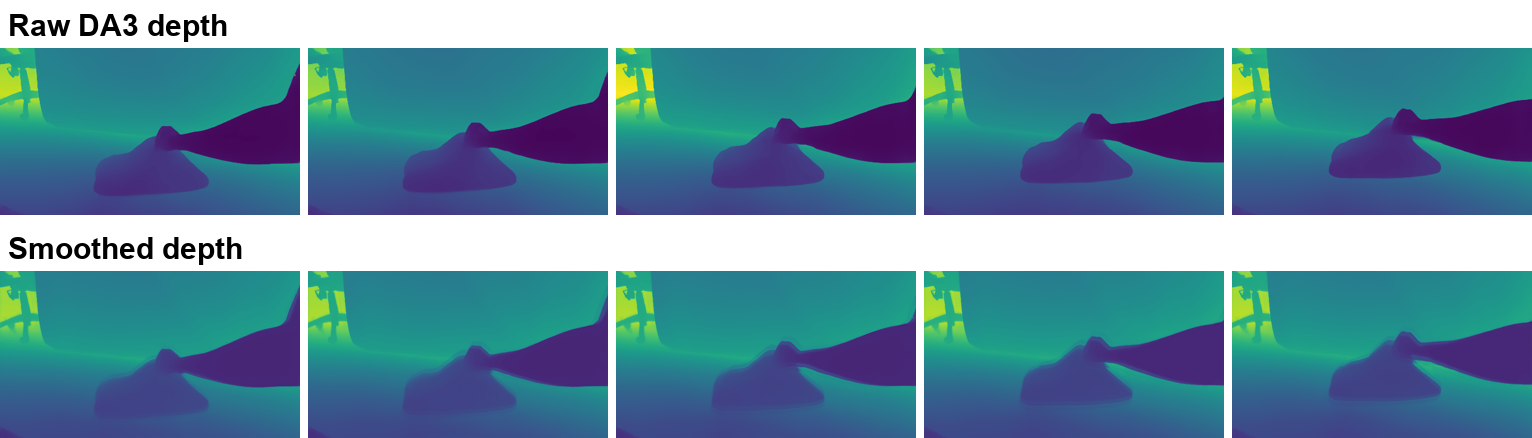
\includegraphics[width = \textwidth]{Images/depth_case_pad}
		\caption{Raw DA3 (top) and smoothed depth (bottom) for five consecutive frames of each
		sequence: sloth stretch, monkey bend and mat lift.}
		\label{fig:eval-depth-cases}
	\end{center}
\end{figure}

\begin{figure}[H]
	\begin{center}
		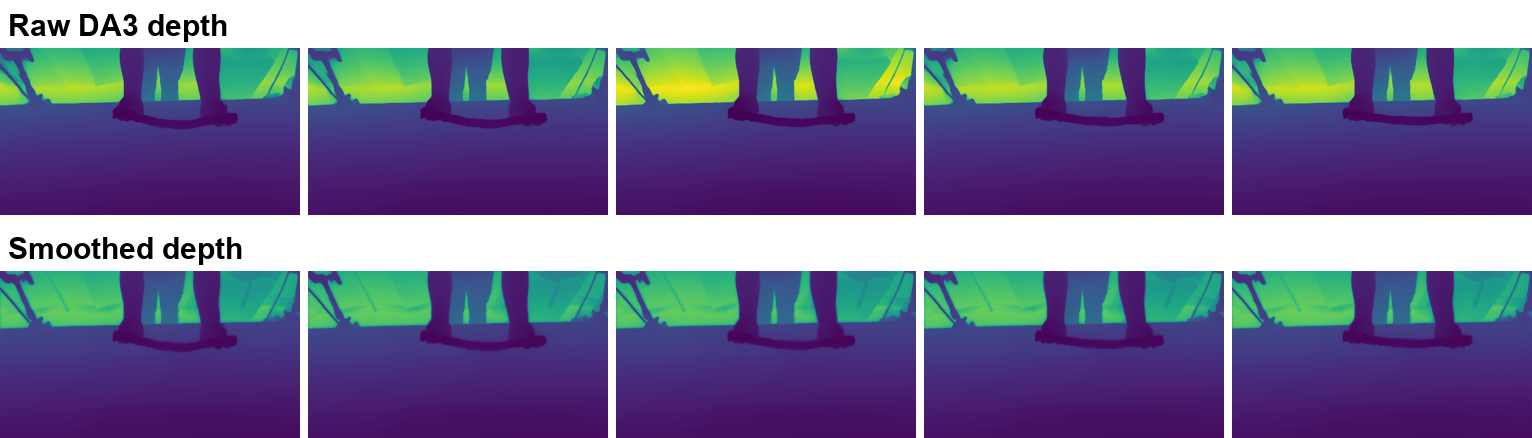
\includegraphics[width = \textwidth]{Images/depth_case_rope}\\
		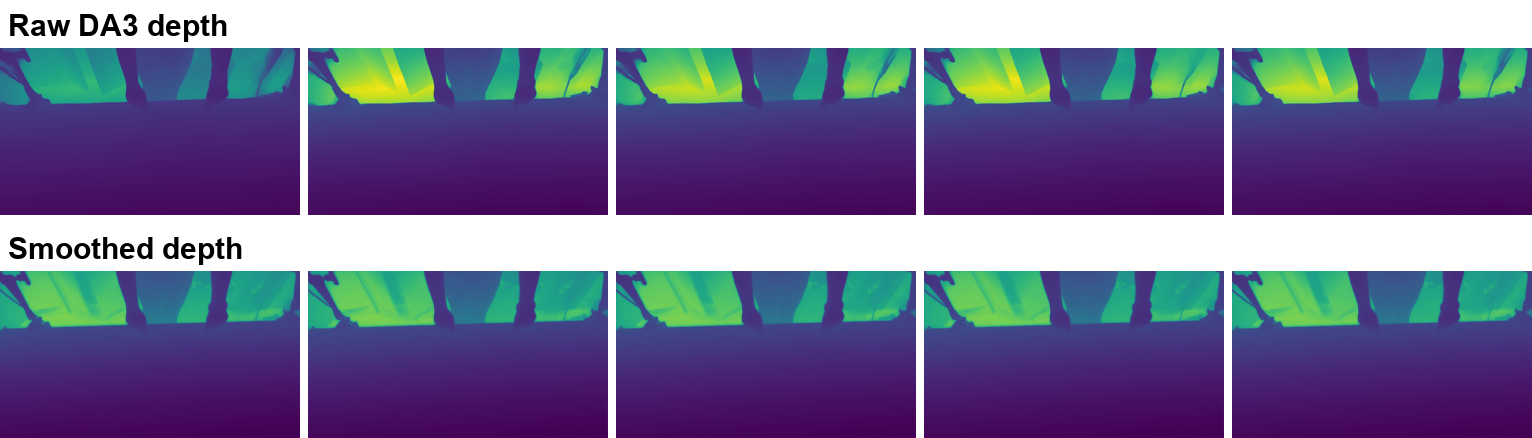
\includegraphics[width = \textwidth]{Images/depth_case_cloth}
		\caption{The same comparison for the rope and cloth sequences.}
		\label{fig:eval-depth-cases-2}
	\end{center}
\end{figure}

\section{Effect on Tracking}
\label{sec:eval-tracking}

The track comparisons ask how much the recovered 3D tracks change between pipeline
variants. Each pair of runs reconstructs the same sequence from differently built input data: either
the depth source differs (the original sensor depth and the new inferred depth), or only the temporal
smoothing of the inferred depth differs. The comparison scripts did not isolate these factors
reliably and reported differences that are not physically plausible: tens of centimetres of
trajectory error between runs whose inputs differ only in the depth treatment. Those figures are
therefore not reported here. The effect of the depth source itself is compared qualitatively in
Section~\ref{sec:eval-ognew}, and the cloth pair below is the clearest example of the effect of
smoothing.

Figure~\ref{fig:eval-track-vis} visualises that cloth pair
(\texttt{single\_lift\_cloth\_3\_new} against \texttt{single\_lift\_cloth\_3\_smooth}), which
differs only in whether the inferred depth was smoothed. The tracked object points of the two runs
overlap almost completely, and the spread and velocity curves show that smoothing the inferred
depth removes frame-to-frame jitter while the recovered motion is preserved.

\begin{figure}[H]
	\begin{center}
		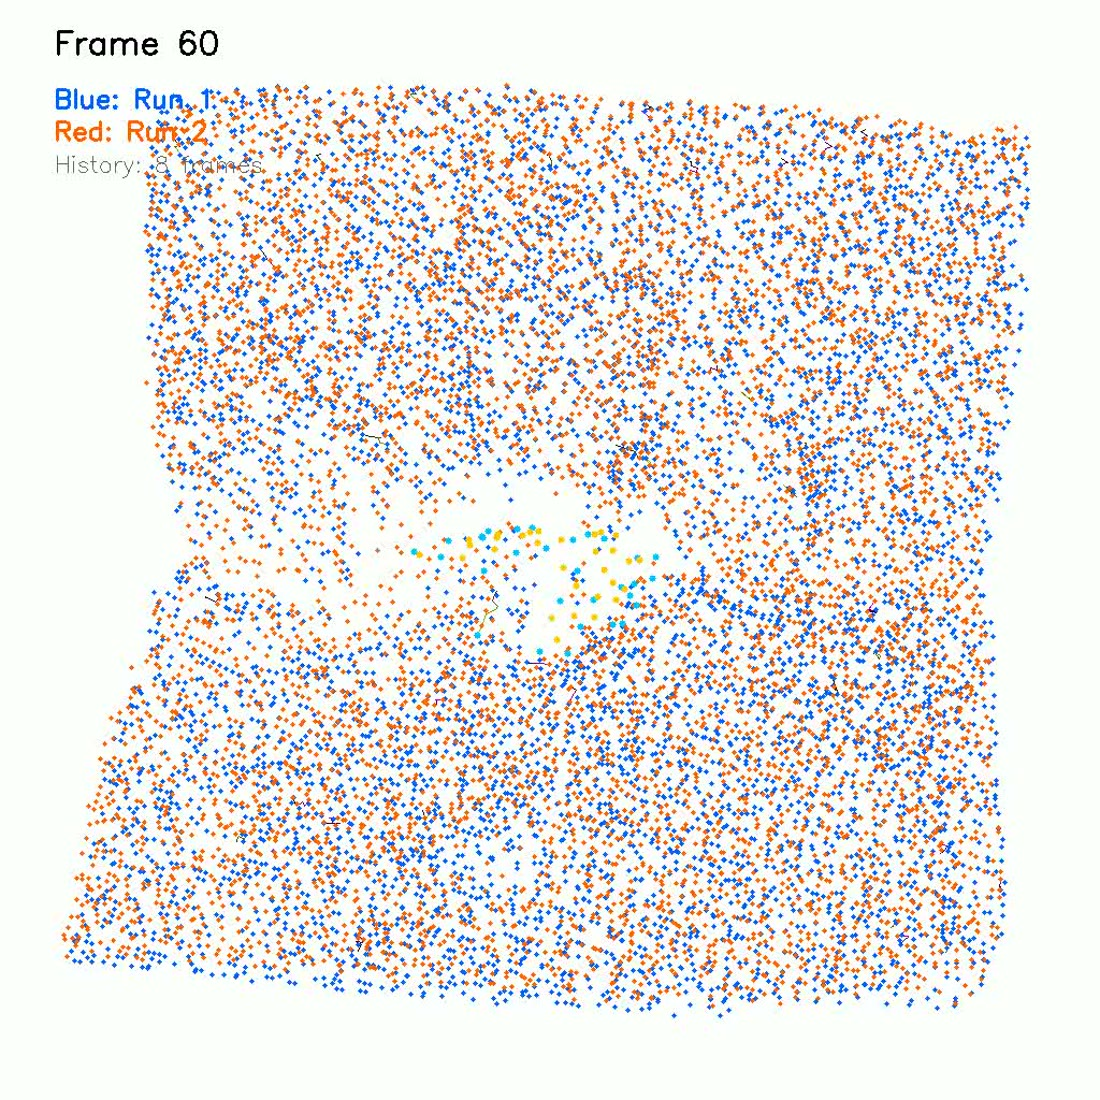
\includegraphics[width = 0.72\textwidth]{Images/track_overlay_ghosts}\\
		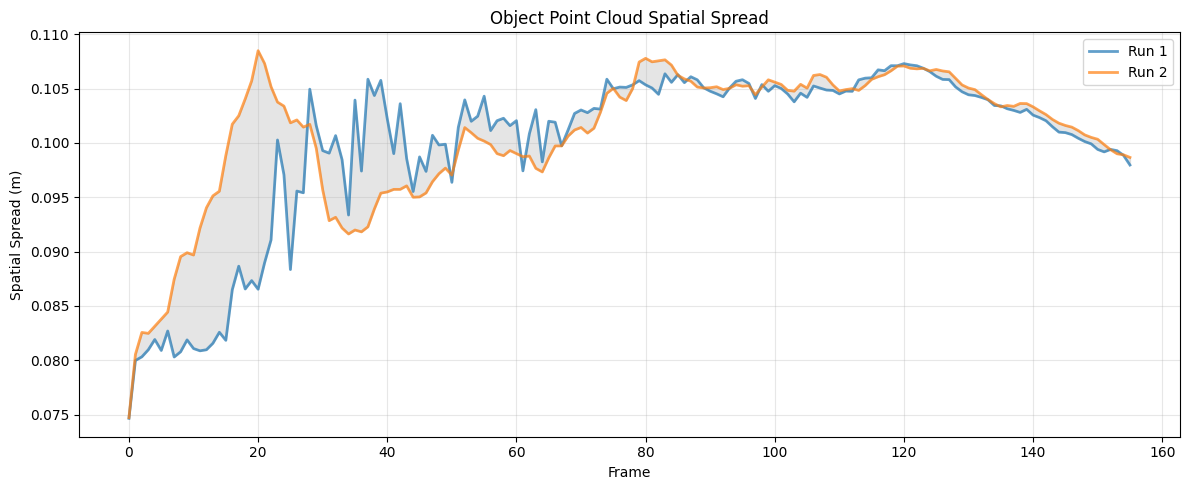
\includegraphics[width = 0.48\textwidth]{Images/track_object_spread}\hfill
		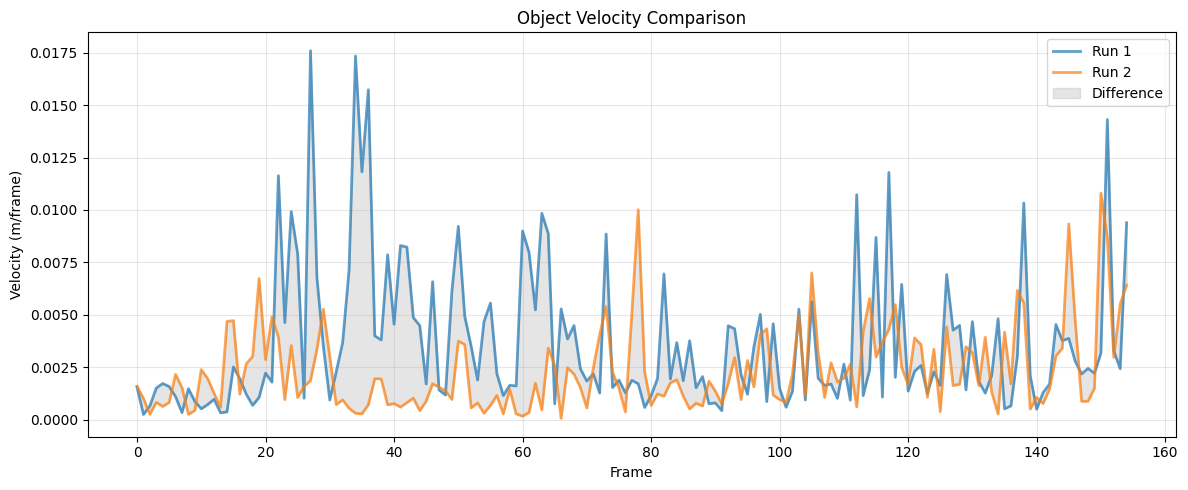
\includegraphics[width = 0.48\textwidth]{Images/track_object_velocity}
		\caption{Tracking for the cloth pair (\texttt{single\_lift\_cloth\_3\_new} against
		\texttt{single\_lift\_cloth\_3\_smooth}). Top: tracked points of both runs overlaid.
		Bottom: object point-cloud spread and velocity; Run 1 unsmoothed, Run 2 smoothed.}
		\label{fig:eval-track-vis}
	\end{center}
\end{figure}

\section{End-to-End Results}
\label{sec:eval-endtoend}

DIPhysTwin completed on PhysTwin and self-collected data and produced interactive spring--mass
warp models. On PhysTwin sequences, the author's visual inspection found the results broadly similar to the RGBD baseline.
All runs use inferred poses, depth and ground alignment.

\begin{figure}[H]
	\begin{center}
		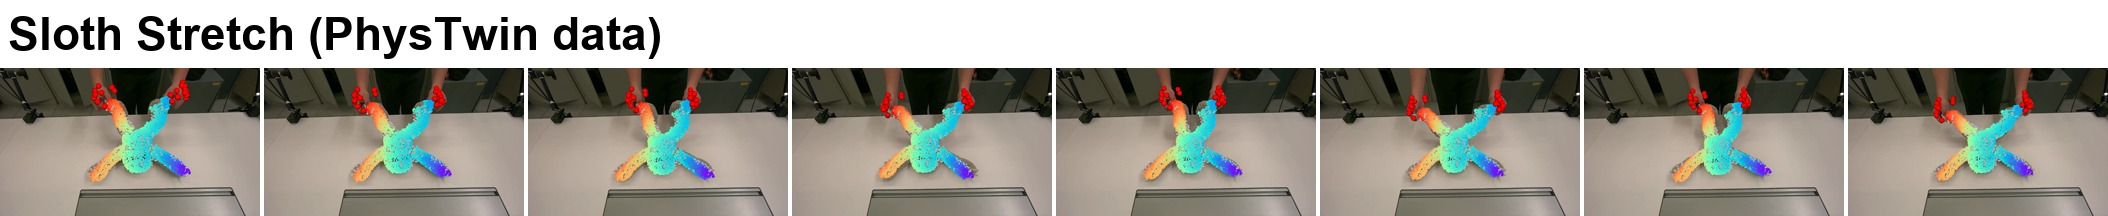
\includegraphics[width = \textwidth]{Images/result_sloth}\\
		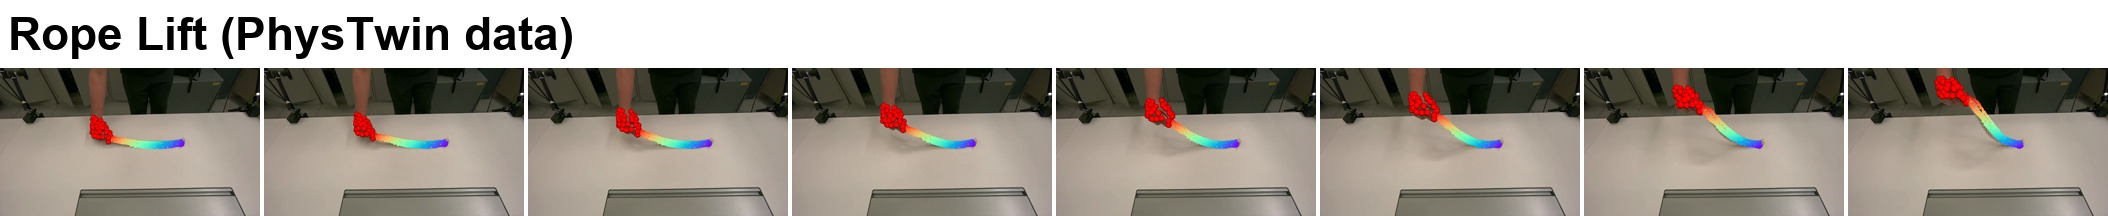
\includegraphics[width = \textwidth]{Images/result_rope}\\
		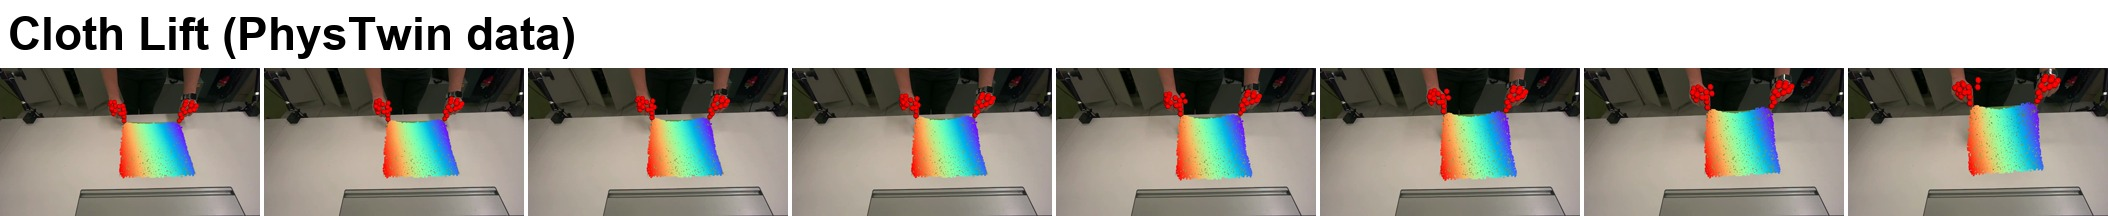
\includegraphics[width = \textwidth]{Images/result_cloth}\\
		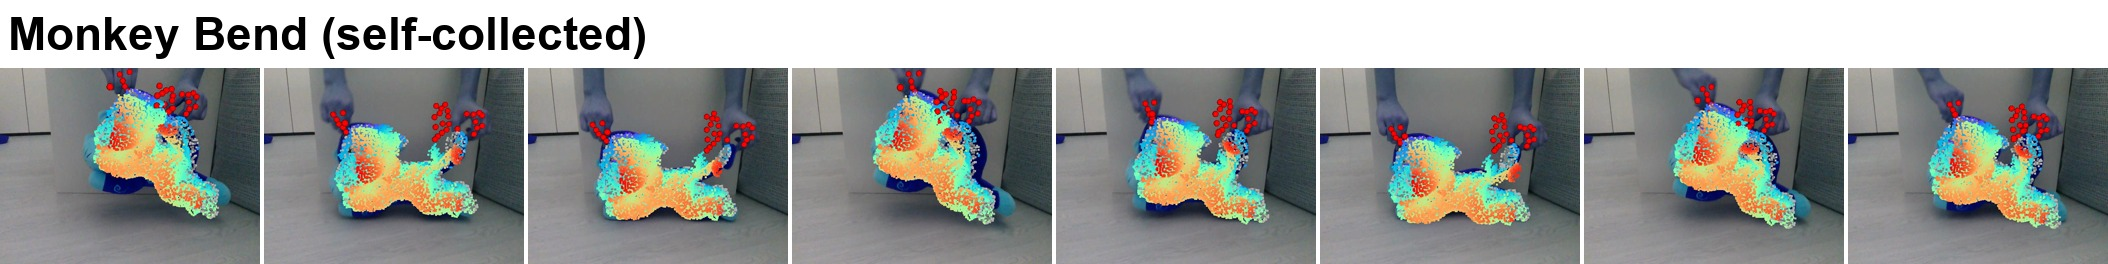
\includegraphics[width = \textwidth]{Images/result_monkey}\\
		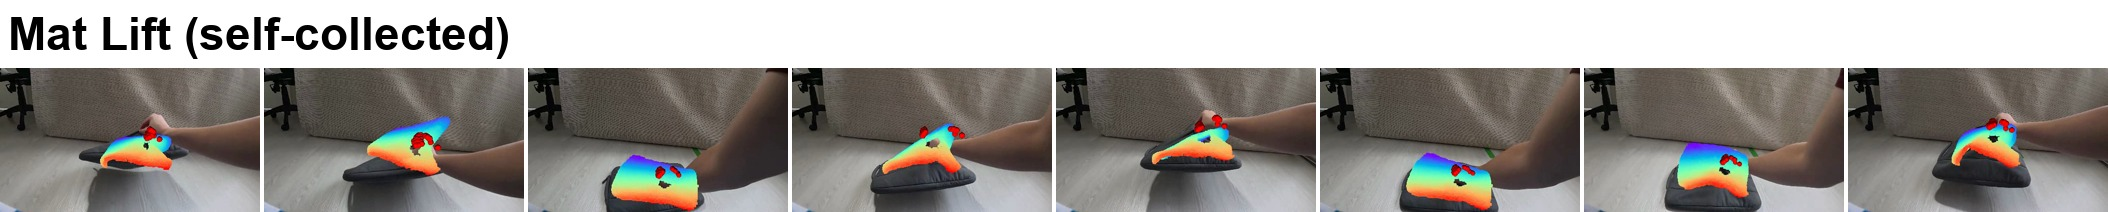
\includegraphics[width = \textwidth]{Images/result_pad}
		\caption{Warp-model results for five objects, eight frames sampled through each clip. Sloth, rope and cloth use PhysTwin data; monkey and mat
		are self-collected.}
		\label{fig:eval-results}
	\end{center}
\end{figure}

Recorded clips of the results are listed in Appendix~\ref{app:results}.

Figure~\ref{fig:eval-results} shows the trained warp models replaying the recorded interactions.
The sloth, cloth and mat rows deform plausibly under the tracked controller motion; the rope row
shows the thin-object case, where the model is driven by few object points. Monkey and mat are
self-collected sessions and complete the pipeline with inferred pose and depth. Mat lift was recorded with looser constraints and still performs reasonably well.

\section{Comparison with the original pipeline}
\label{sec:eval-ognew}

Figure~\ref{fig:eval-ognew} compares the trained warp models of the original PhysTwin pipeline,
which uses the sensor depth, with DIPhysTwin, which uses inferred depth, on the same sequences
and at the same times; Figure~\ref{fig:eval-ognew-2} shows the self-collected monkey and mat sequences. For the monkey and mat pairs, re-captured sessions use recorded depth values, while retraining uses smoothed inferred depth. The
sloth sequence is shown stage by stage in Appendix~\ref{sec:app-vid-sloth-chain}.

\begin{figure}[H]
	\begin{center}
		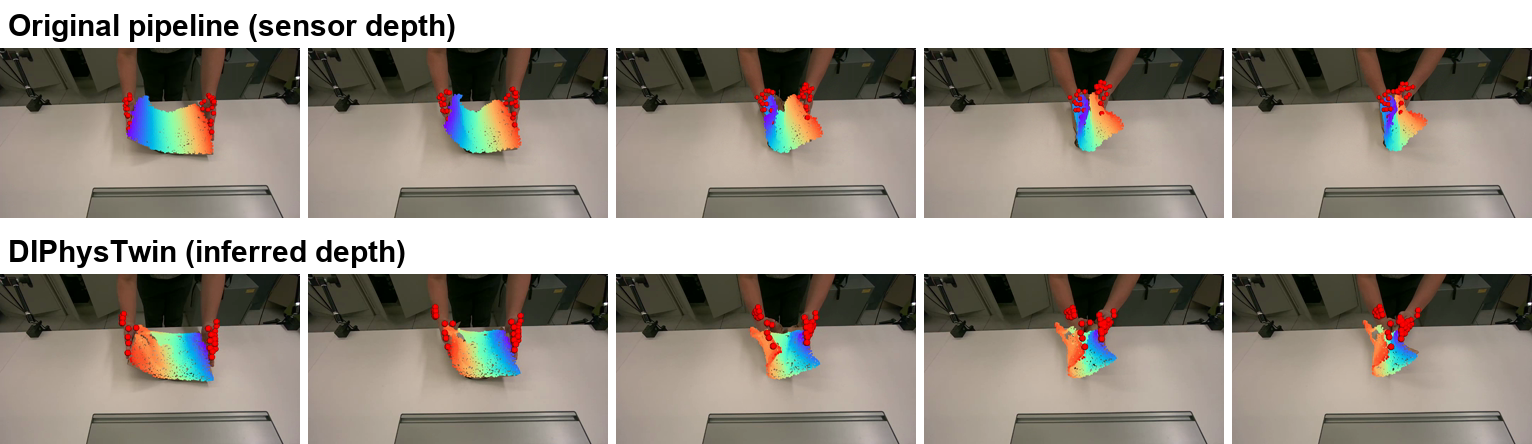
\includegraphics[width = \textwidth]{Images/ognew_package}\\
		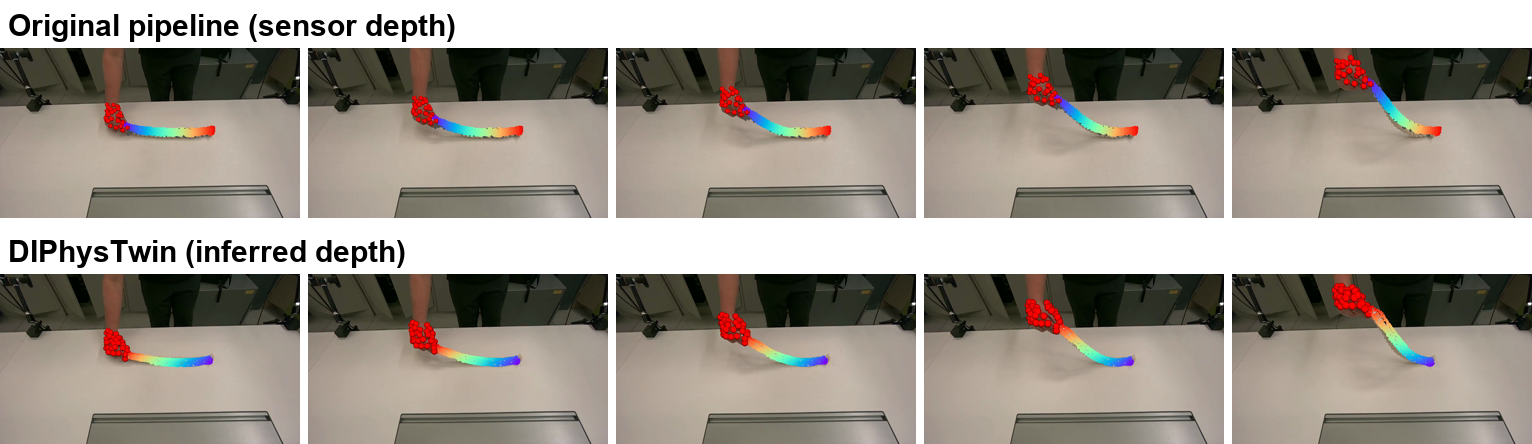
\includegraphics[width = \textwidth]{Images/ognew_rope}\\
		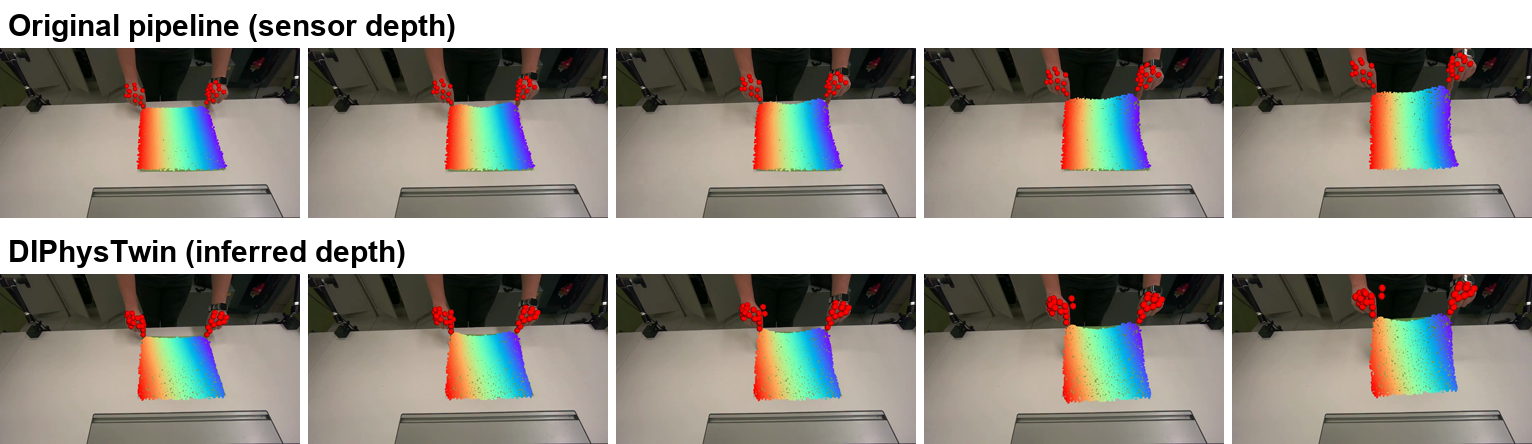
\includegraphics[width = \textwidth]{Images/ognew_cloth}
		\caption{Original PhysTwin pipeline (top row of each object, sensor depth) against
		DIPhysTwin (bottom row, inferred depth) on the package, rope and cloth sequences, at matched
		times.}
		\label{fig:eval-ognew}
	\end{center}
\end{figure}

\begin{figure}[H]
	\begin{center}
		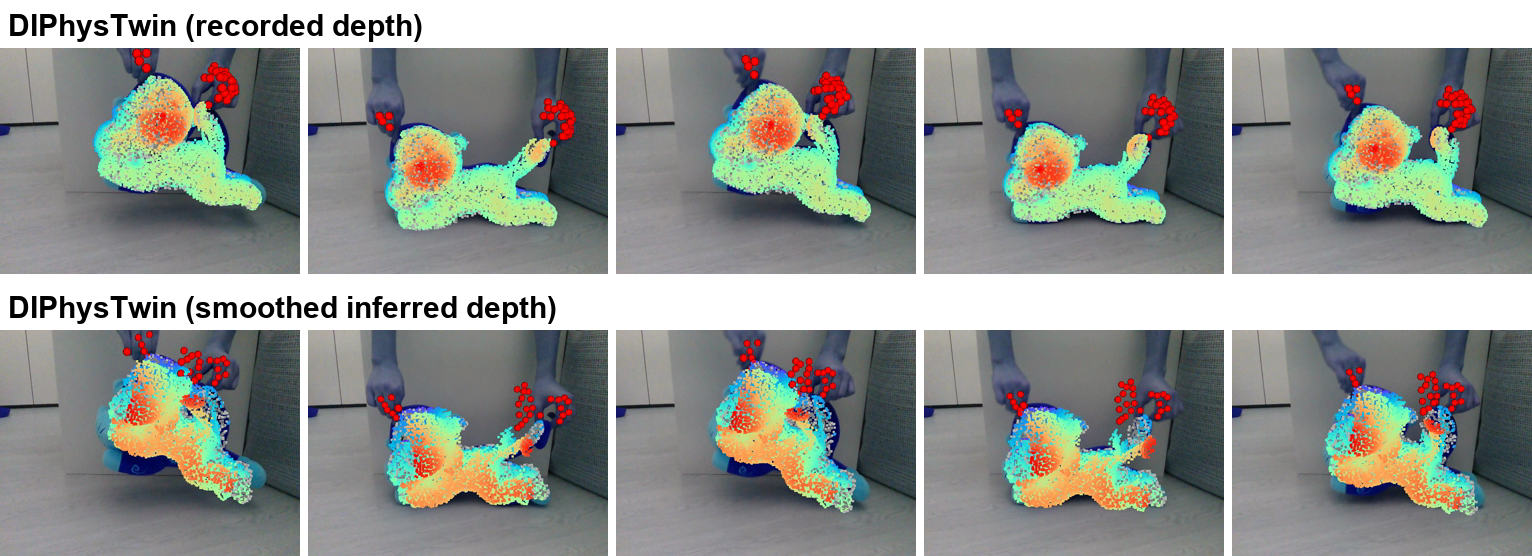
\includegraphics[width = \textwidth]{Images/ognew_monkey}\\
		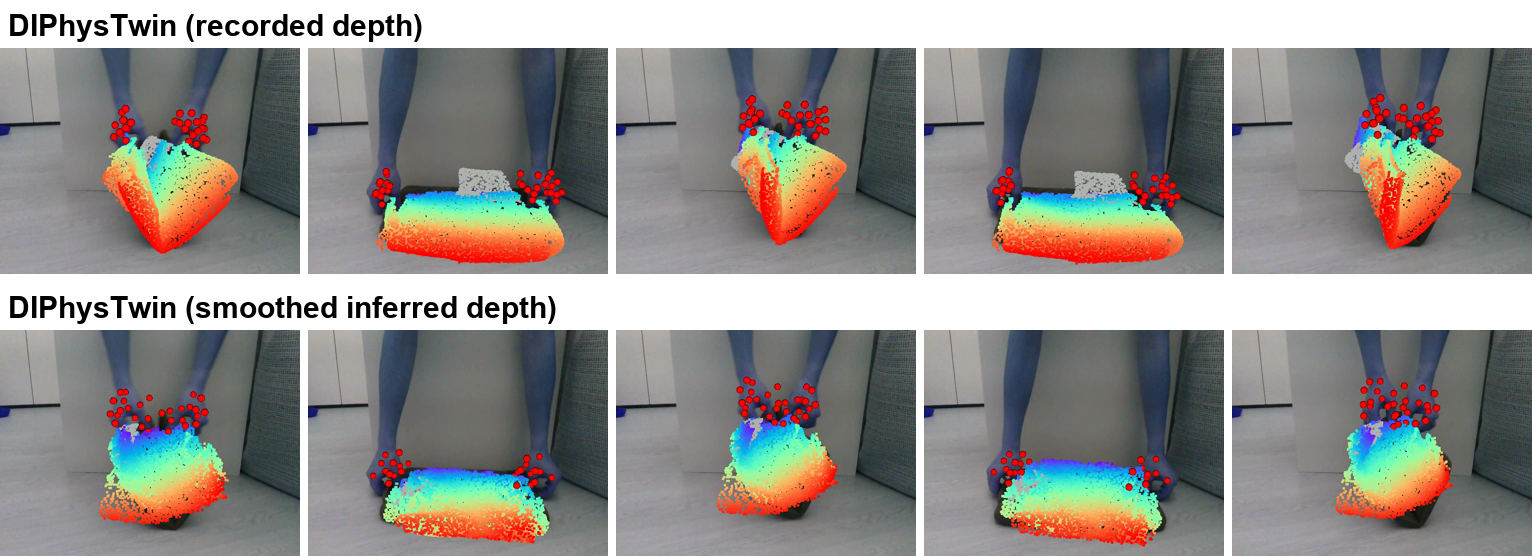
\includegraphics[width = \textwidth]{Images/ognew_pad}
		\caption{The monkey (stuffed animal) and mat sequences. Top row: DIPhysTwin runs with recorded depth; bottom row: runs with smoothed inferred depth.}
		\label{fig:eval-ognew-2}
	\end{center}
\end{figure}

The two rows are hard to compare cleanly. The inferred-depth runs still show jitter and 3D
inconsistency, and these artefacts affect training overall. The two pipelines also differ in other
respects, so the figure does not isolate how much of any difference comes from the depth source alone.

\section{Findings and Failure Cases}
\label{sec:eval-findings}

Large, slow-moving objects with little occlusion reconstructed reliably. Heavy controller
occlusion damaged segmentation, shape-prior generation and tracking. Small, fast-moving objects
showed unstable depth and weaker 3D consistency; recovery also deteriorated when controller contact
was lost. Spatial coherence weakened over time, especially in early unsynchronised captures, and
unusual rotations reconstructed poorly. Soft objects without ground support required excessive
stiffness before ground alignment was corrected; Appendix~\ref{sec:app-vid-ground} shows the rope
sequence before and after the correction.

\begin{table}[H]
	\caption{The author's qualitative assessment of capture conditions and outcome across the self-collected sessions. Outcomes are not counted per session.}
	\label{tab:eval-objects}
	\begin{center}
		\begin{tabular}{@{}>{\raggedright\arraybackslash}p{2.6cm}
		                  >{\raggedright\arraybackslash}p{2.2cm}
		                  >{\raggedright\arraybackslash}p{2.3cm}
		                  >{\raggedright\arraybackslash}p{3.0cm}
		                  >{\raggedright\arraybackslash}p{2.5cm}@{}}
			\toprule
			Object & Scale & Motion speed & Controller occlusion & Outcome \\
			\midrule
			Mat or foam pad & Large & Slow & Minimal & Good \\
			Stuffed animal & Moderate & Slow & Minimal & Good \\
			Cloth & Large & Fast & Significant & Partial \\
			Bottle & Small & Fast & Significant & Poor \\
			Mug & Small & Fast & Significant & Poor \\
			Rope & Large, thin & Slow & None (no ground support) & Partial \\
			\bottomrule
		\end{tabular}
	\end{center}
\end{table}

% The original PhysTwin data is summarised in Table~\ref{tab:phystwin-data} (Chapter~\ref{cha:system-design}).

\section{Negative Results}
\label{sec:eval-negative}

Different tools and methodologies were also tested but did not improve the pipeline. The following list is not exhaustive, but it covers the main alternatives that were tried and abandoned.

Replacing DA3 with $\pi^3$ failed to preserve alignment with known camera poses \parencite{pi3}.
MVTracker performed worse than 2D tracking, while SpatialTrackerV2 produced frequent 3D artefacts
\parencite{mvtracker, spatrackerv2} (Appendix~\ref{sec:app-vid-spatracker}). Trellis and the current CoTracker version gave no
visible improvement \parencite{trellis, cotracker}. Inference without chunk stitching was also tested; its recordings are listed in
Appendix~\ref{sec:app-vid-streaming}.
 
\chapter{Discussion, Limitations and Future Work}\label{cha:discussion}
\label{cha:conclusion}

\section{Summary and Diagnosis}
\label{sec:disc-diagnosis}\label{sec:concl-summary}

DIPhysTwin adapts PhysTwin to multi-view RGB video: camera poses, depth and ground alignment are
inferred, then handed to its reconstruction and warp-model stages. The new component is a residual
depth smoother, supervised by Video Depth Anything (VDA) as a motion oracle and trained without
ground-truth depth \parencite{phystwin, vda}.

The pipeline is still 2D-first: segmentation and CoTracker run on RGB, and depth lifts their output
into 3D \parencite{cotracker}. Depth errors therefore reach the tracks, the shape prior, the
reconstruction and the warp model at once. No tested depth model was good at both jobs. DUSt3R,
MASt3R and DA3 give geometry but flicker, while VDA is smooth but monocular and geometrically weak
\parencite{dust3r, mast3r, da3, vda}. The smoother takes geometry from the first group and motion
from the second, at the cost of some blur (Chapter~\ref{cha:evaluation}).

Two alternatives were considered and dropped. Replacing the weak parts of the PhysTwin pipeline
with a multi-pose streaming depth model and multi-view tracking would require a new model
\parencite{dust3r, mast3r, cotracker}. Rewriting around 4D Gaussian splatting would remove explicit
poses but move segmentation and tracking into 3D \parencite{fourdgs, gaussiansplatting}.
\label{sec:disc-alternatives}

\section{Limitations}
\label{sec:disc-limitations}

The depth stage is not truly streaming. Duplicating fixed views as a dynamic sequence helps only
over short windows; larger chunks make the Umeyama alignment singular \parencite{umeyama1991}. The
three cameras also differ in intrinsics and distortion, use rolling shutters and automatic exposure
and focus, and were never time-synchronised; software only aligned their start times. The later rig
used measured intrinsics and extrinsics only as a reference, and may still be slightly fisheye. These conditions explain
the observed symptoms: flicker, spatial drift within a clip, and failures on fast motion and unusual
rotations. \label{sec:disc-streaming}\label{sec:disc-data}

The environment is static. The floor collider fixed the over-stiff behaviour for supported
objects, but a rope has little ground support and still needs unrealistic stiffness. The smoother
blurs depth, and the current evaluation cannot say whether it removes flicker without also removing
fine geometry. \label{sec:disc-environment}\label{sec:disc-smoothing}

The depth comparison covers one sequence, the remaining evidence is qualitative, and the loss
weights are untuned. The findings on object size, speed and occlusion are observed trends from a small number of sessions.
\label{sec:disc-validity}

\section{Future Work}
\label{sec:concl-future}

The depth stage needs true multi-view streaming. A model that accepts several camera poses would
replace the chunk-overlap workaround and its unstable alignment \parencite{umeyama1991}. The same
model should be both spatially consistent and temporally smooth, and the shape prior needs to handle
non-watertight meshes \parencite{arap}. \label{sec:concl-streaming}\label{sec:concl-depth}

The capture should be repeated with synchronisation cues, locked exposure and focus, and measured
intrinsics, allowing for fisheye distortion.
Tracking needs to survive occlusion and partially visible objects; MVTracker and direct 3D tracking
are the next candidates \parencite{mvtracker, spatrackerv2}. Environment interaction
should move from static planes to moving rigid bodies. \label{sec:concl-data}\label{sec:concl-tracking}\label{sec:concl-environment}

The smoother needs loss-term and span ablations, multi-view evaluation, and comparison against
reference geometry where any exists. After that the pipeline should be cleaned up and released.
\label{sec:concl-code}

\section{Conclusion}
\label{sec:concl-closing}

DIPhysTwin turns multi-view RGB video into an interactive digital twin, and the smoother reduces
temporal flicker without ground-truth depth. Results are strongest for large, slow-moving
objects under controlled capture. Depth coherence, occlusion, calibration and tracking remain the
main limitations.
 


% ------------------------------------------------------------------------------
% Reference list
% ------------------------------------------------------------------------------
\addcontentsline{toc}{chapter}{References}
\renewcommand\bibname{References}
\printbibliography

% ------------------------------------------------------------------------------
% Appendices
% ------------------------------------------------------------------------------
\appendix

\chapter{Extended Results and Result Videos}
\label{app:results}

The recordings below accompany this report. They are grouped by what they compare: within each
comparison table one row shows the same scene under two or more pipeline variants, so the effect of
a single change can be seen directly. Scene names describe the captured interaction (for example
``cloth, single lift'' is a cloth lifted from one point). Recording links are given in shortened
form.

\section{Improvement Chain on the Sloth Sequence}
\label{sec:app-vid-sloth-chain}

Table~\ref{tab:app-vid-sloth} shows the improvement chain on the sloth sequence: the original
pipeline (sensor reference depth), the pipeline with DA3 inferred depth, and the pipeline with
smoothed DA3 depth. Each stage replaces one component of the previous one. The measurements in
Chapter~\ref{cha:evaluation} quantify the last step: for this sequence the smoothed depth keeps the
agreement with the sensor reference (Spearman 0.988, ordinal error 3.3\% on camera 0) with a higher
gradient correlation than raw DA3 (0.169 against 0.117; Table~\ref{tab:eval-depth-sensor}).

\begin{table}[H]
    \caption{Sloth sequence: the three pipeline stages.}
    \label{tab:app-vid-sloth}
    \begin{center}
        \small
        \begin{tabular}{@{}p{6.2cm}l@{}} \toprule
            Stage & Recording \\ \midrule
            1. Original pipeline (reference depth) & \url{youtu.be/UyQw7Hx25D8} \\
            2. DA3 inferred depth with streaming   & \url{youtu.be/Wldxhw5DKHs} \\
            3. Smoothed DA3 inferred depth         & \url{youtu.be/xjoEsQoWlXw} \\ \bottomrule
        \end{tabular}
    \end{center}
\end{table}

\section{Effect of the Temporal Depth Smoother}
\label{sec:app-vid-smoother}

\paragraph{Raw DA3 depth against smoothed depth.}
\label{sec:app-vid-raw}

Each row of Table~\ref{tab:app-vid-raw} shows one scene twice: the raw DA3 depth prediction and the
same frames after temporal smoothing. The raw recordings show the frame-to-frame flicker that
motivates the smoother (Chapter~\ref{cha:smoother}): the depth of static surfaces shifts between
consecutive frames and the object--background boundary moves.

\begin{table}[H]
    \caption{Raw DA3 depth against smoothed depth.}
    \label{tab:app-vid-raw}
    \begin{center}
        \small
        \begin{tabular}{@{}p{3.4cm}ll@{}} \toprule
            Scene & Raw DA3 depth & Smoothed depth \\ \midrule
            Cloth, single lift & \url{youtu.be/c_K8Iw4v8GM} & \url{youtu.be/Oix-bPoGo1Y} \\
            Zebra, double lift & \url{youtu.be/22x_s_dwmJA} & \url{youtu.be/jrlRHbfc8wo} \\
            Mat, single lift   & \url{youtu.be/CfmDhliW4e4} & \url{youtu.be/eaA4PYEcdmU} \\ \bottomrule
        \end{tabular}
    \end{center}
\end{table}

\paragraph{Pipeline replay before and after smoothing.}
\label{sec:app-vid-smooth}

Table~\ref{tab:app-vid-smooth} shows the pipeline replay of the same two scenes before and after
the inferred depth was smoothed, at matched times.

\begin{table}[H]
    \caption{Pipeline replay before and after depth smoothing.}
    \label{tab:app-vid-smooth}
    \begin{center}
        \small
        \begin{tabular}{@{}p{3.4cm}ll@{}} \toprule
            Scene & Before smoothing & After smoothing \\ \midrule
            Cloth, single lift  & \url{youtu.be/oMyWfrkThjA} & \url{youtu.be/sFhpqg2umsA} \\
            Sloth, double stretch & \url{youtu.be/Pyi-6zr_SVY} & \url{youtu.be/DJOm86ircG4} \\ \bottomrule
        \end{tabular}
    \end{center}
\end{table}

\section{Depth-Source Variants}
\label{sec:app-vid-depth-variants}

Table~\ref{tab:app-vid-variants} lists further depth sources used for the same inference
comparison. The reference and DA3 rows repeat the first two stages of
Table~\ref{tab:app-vid-sloth} so that the set is self-contained.

\begin{table}[H]
    \caption{Inference with alternative depth sources.}
    \label{tab:app-vid-variants}
    \begin{center}
        \small
        \begin{tabular}{@{}p{4.6cm}ll@{}} \toprule
            Depth source & Recording & Notes \\ \midrule
            Reference (sensor depth) & \url{youtu.be/UyQw7Hx25D8} & original pipeline \\
            DA3 inferred depth with streaming & \url{youtu.be/Wldxhw5DKHs} & adopted depth source \\
            VDA                      & \url{youtu.be/GUog6wd8YiI} & video model oracle \\
            Without streaming        & \url{youtu.be/NbU0TzVzMGM} & without chunk stitching \\ \bottomrule
        \end{tabular}
    \end{center}
\end{table}

\section{Streaming Inference}
\label{sec:app-vid-streaming}

Table~\ref{tab:app-vid-streaming} compares depth inference with and without chunk stitching
(streaming), for the final data and the final matching visualisations, with a reference recording
of the final data.

\begin{table}[H]
    \caption{Streaming inference against non-streaming inference.}
    \label{tab:app-vid-streaming}
    \begin{center}
        \small
        \begin{tabular}{@{}p{3.4cm}lll@{}} \toprule
            Visualisation & Without streaming & With streaming & Reference \\ \midrule
            Final data & \url{youtu.be/wtfQiYJZQfQ} & \url{youtu.be/b3FfEog8buc} & \url{youtu.be/bH6H2vx3Q4k} \\
            Final matching & \url{youtu.be/m4g420lpaH4} & \url{youtu.be/M2VwlY6B9j4} & --- \\ \bottomrule
        \end{tabular}
    \end{center}
\end{table}

\section{Tracking Comparison with SpatialTrackerV2}
\label{sec:app-vid-spatracker}

Table~\ref{tab:app-vid-spatracker} compares the tracked result of the same monkey sequence with the
2D-tracking-based pipeline and with SpatialTrackerV2 \parencite{spatrackerv2}.

\begin{table}[H]
    \caption{Monkey sequence: DIPhysTwin against SpatialTrackerV2.}
    \label{tab:app-vid-spatracker}
    \begin{center}
        \small
        \begin{tabular}{@{}p{3.6cm}ll@{}} \toprule
            Variant & Recording & Notes \\ \midrule
            DIPhysTwin & \url{youtu.be/8WwHEsOErsI} & spatial separation on fast movement \\
            SpatialTrackerV2 & \url{youtu.be/DijnnXjS_Xc} & frequent 3D artefacts \\ \bottomrule
        \end{tabular}
    \end{center}
\end{table}

\section{Environment Interaction: Rope with and without Ground Alignment}
\label{sec:app-vid-ground}

Table~\ref{tab:app-vid-ground} shows the rope sequence before and after the ground-plane alignment
was added (Chapter~\ref{cha:system-design}), together with the reference recording of the same
interaction.

\begin{table}[H]
    \caption{Rope sequence: stiff result, reference interaction, and recovered ground contact.}
    \label{tab:app-vid-ground}
    \begin{center}
        \small
        \begin{tabular}{@{}p{5.2cm}ll@{}} \toprule
            Variant & Recording & Notes \\ \midrule
            Without ground alignment & \url{youtu.be/I59sUpi_Rvk}  & rope overly stiff \\
            Reference interaction    & \url{youtu.be/fhun0051Rps}  & rope rests on the ground \\
            With ground alignment    & \url{youtu.be/zXyEl8aMBYk}  & ground contact recovered \\ \bottomrule
        \end{tabular}
    \end{center}
\end{table}

\section{Individual Demonstrations}
\label{sec:app-vid-solo}

Single recordings without a paired comparison, grouped by type.

\begin{table}[H]
    \caption{Individual demonstration recordings.}
    \label{tab:app-vid-solo}
    \begin{center}
        \small
        \begin{tabular}{@{}llp{4.6cm}@{}} \toprule
            Recording & Scene & Notes \\ \midrule
            \multicolumn{3}{@{}l}{\emph{Tracking results}} \\
            \url{youtu.be/94h6tWvJEwE} & Mat, double bend & tracking reconstruction \\
            \url{youtu.be/ICQz9aUabAo} & Mat, single lift & tracking reconstruction \\ \midrule
            \multicolumn{3}{@{}l}{\emph{Pipeline demonstrations, PhysTwin data}} \\
            \url{youtu.be/nsndv85sxcU} & Sloth, double stretch & \\
            \url{youtu.be/t97kz2DZZxk} & Zebra, double lift & \\
            \url{youtu.be/wVsCuG4sxWI} & Cloth, double hand lift & \\
            \url{youtu.be/FUNXNBtAupQ} & Cloth, single lift & degraded result \\
            \url{youtu.be/I59sUpi_Rvk} & Rope, single lift & see Table~\ref{tab:app-vid-ground} \\ \midrule
            \multicolumn{3}{@{}l}{\emph{Pipeline demonstrations, self-collected data}} \\
            \url{youtu.be/U8ICkg25_4U} & Mat, double bend & \\
            \url{youtu.be/rtjAy8hZE8k} & Mat, single lift & \\
            \url{youtu.be/RTn-0Zg8wAA} & Water bottle, single lift & poor result \\
            \url{youtu.be/SbAI6K0lMDk} & T-shirt, single lift & \\
            \url{youtu.be/svUzZCJdgDk} & Monkey, double bend & \\
            \url{youtu.be/yZ0TzMy9XA0} & Package, single lift & \\ \midrule
            \multicolumn{3}{@{}l}{\emph{New-data captures, three camera corners}} \\
            \url{youtu.be/sFbwJNk7rUs} & Mat, single lift & camera corner 0 \\
            \url{youtu.be/LdueFxEb7H8} & Mat, single lift & camera corner 1 \\
            \url{youtu.be/ZcDswgNRI40} & Mat, single lift & camera corner 2 \\ \midrule
            \multicolumn{3}{@{}l}{\emph{Issue and failure recordings}} \\
            \url{youtu.be/e6UjWpdsnjg} & Mat, double bend & object split during interaction \\
            \url{youtu.be/8WwHEsOErsI} & Monkey, double bend & see Table~\ref{tab:app-vid-spatracker} \\
            \url{youtu.be/4lE1MX_xUnM} & Rope, single lift & depth flicker propagating into 3D tracks \\ \midrule
            \multicolumn{3}{@{}l}{\emph{Further recordings}} \\
            \url{youtu.be/TVVKJ1hBin8} & Sloth, double stretch & interactive playground session \\
            \url{youtu.be/cywRH67oSGY} & Sloth, double stretch & depth-quality comparison with metrics \\
            \url{youtu.be/R-0QuXLqUTQ} & Mat, double bend & early result, poor \\
            \url{youtu.be/44K07VyE1iI} & Mat, single lift & early result \\ \bottomrule
        \end{tabular}
    \end{center}
\end{table}

\chapter{Hyper-parameters and Loss Weights}
\label{app:hyperparameters}

This appendix records the settings needed to reproduce the temporal depth smoother. The values
are the training configurations saved with the checkpoints.

\begin{table}[H]
    \caption{Training and inference hyper-parameters of the reported smoother run.}
    \label{tab:app-hyperparameters}
    \begin{center}
        \begin{tabular}{@{}p{3.6cm}p{10.4cm}@{}}
            \toprule
            Setting & Value \\
            \midrule
            Optimiser & Adam; weight decay $10^{-4}$ \\
            Learning rate & $3\times10^{-3}$ \\
            Schedule & ReduceLROnPlateau; factor $0.5$, patience 5 \\
            Batch size & 2 \\
            Epochs & 50; checkpoints saved for epochs 0--49 \\
            Precision & CUDA autocast with bfloat16 \\
            Hardware & NVIDIA GeForce RTX 3060 \\
            Inference chunk length & 16 frames per chunk, matching the training window; chunks
            overlap and are blended with a weighted window \\
            \bottomrule
        \end{tabular}
    \end{center}
\end{table}

\begin{table}[H]
    \caption{Loss weights of the best saved smoother runs; the first row is the run behind the
    reported results. $\lambda_{\mathrm{edge}}$ and $\lambda_{\mathrm{grad}}$ are the
    edge-sharpness and spatial-gradient terms of Section~\ref{sec:smoother-losses}.}
    \label{tab:app-lossweights}
    \begin{center}
        \small
        \begin{tabular}{@{}p{5.6cm}ccccc@{}}
            \toprule
            Run & $\lambda_{\mathrm{fid}}$ & $\lambda_{\mathrm{tgm}}$ & $\lambda_{\mathrm{tv}}$
            & $\lambda_{\mathrm{edge}}$ & $\lambda_{\mathrm{grad}}$ \\
            \midrule
                        \texttt{best\_model} & 1.2 & 0.5 & 0.5 & 0.3 & 0 \\
            \texttt{best\_model\_50\_epochs} & 1.2 & 0.5 & 0.5 & 0.3 & 0 \\
            \texttt{best\_model\_50\_epochs\_no\_edge\_blur} & 1.3 & 0.8 & 0.8 & 0.05 & 0.04 \\
            \texttt{best\_model\_new\_data} & 1.3 & 0.8 & 0.8 & 0.05 & 0.05 \\
            \bottomrule
        \end{tabular}
    \end{center}
\end{table}

The temporal spans follow the code defaults used by all runs: TGM $k = 1, 2, 3$ with weights
$1, 0.25, 0.07$, and TV $k = 1, 2$ with weights $1, 0.25$.



\chapter{Source Code}
\label{app:code}

The implementation is released at
\url{https://github.com/Hanson-Sun/PhysTwin/tree/depth-inference-phystwin}.



\end{document}